% Created 2026-05-20 qua 22:23
% Intended LaTeX compiler: xelatex
\documentclass[12pt,a4paper]{article}
\usepackage{graphicx}
\usepackage{longtable}
\usepackage{wrapfig}
\usepackage{rotating}
\usepackage[normalem]{ulem}
\usepackage{capt-of}
\usepackage{hyperref}
\usepackage[T1]{fontenc}
\usepackage[utf8]{inputenc}
\usepackage[brazil, brazilian]{babel}
\usepackage[top=2.5cm,bottom=2.5cm,left=3cm,right=2.5cm]{geometry}
\usepackage{lmodern}
\usepackage{microtype}
\usepackage{minted}
\setminted{fontsize=\small, linenos=false, breaklines=true, bgcolor=gray!6}
\usepackage[colorlinks=true, linkcolor=black, urlcolor=blue, citecolor=black]{hyperref}
\usepackage{fancyhdr}
\pagestyle{fancy}
\fancyhf{}
\fancyhead[L]{\small Ciência de Dados - Laboratório 6}
\fancyhead[R]{\small Análise Exploratória de Dados e Engenharia de Features}
\fancyfoot[C]{\thepage}
\renewcommand{\headrulewidth}{0.4pt}
\usepackage{setspace}
\setstretch{1.15}
\usepackage{fancyvrb}
\usepackage{etoolbox}
\usepackage{fancyvrb}
\DefineVerbatimEnvironment{Highlighting}{Verbatim}{commandchars=\\\{\}, formatcom=\small\color{gray}, frame=single, framesep=5mm, rulecolor=\color{lightgray}}
\usepackage{minted}
\usepackage{xcolor}
\definecolor{lightgray}{gray}{0.95}
\setminted{style=vs, fontsize=\small, frame=single, bgcolor=lightgray}
\AtBeginDocument{\setlength{\parskip}{4pt}}
\author{Nícolas Rosenthal Dal Corso}
\date{\date}
\title{Laboratório 6 - Análise Exploratória de Dados e Engenharia de \emph{Features}}
\hypersetup{
 pdfauthor={Nícolas Rosenthal Dal Corso},
 pdftitle={Laboratório 6 - Análise Exploratória de Dados e Engenharia de \emph{Features}},
 pdfkeywords={},
 pdfsubject={},
 pdfcreator={Emacs 30.2 (Org mode 9.7.11)}, 
 pdflang={Portuges}}
\begin{document}

\maketitle
\setcounter{tocdepth}{3}
\tableofcontents

\section{Análise Exploratória dos Dados}
\label{sec:org630f56d}
\subsection{Tecnologias Utilizadas}
\label{sec:org141cb82}
Para a análise exploratória dos dados (EDA, \emph{exploratory data analysis}) do conjunto de dados \href{https://www.kaggle.com/competitions/spaceship-titanic}{Spaceship Titanic} será utilizada linguagem de programação R, historicamente construída para, principalmente, análise estatística, e a coleção de pacotes \href{https://tidyverse.org/}{tidyverse}, integrados ao \href{https://orgmode.org/}{org-mode}, \emph{major mode} para \emph{literate programming} já plenamente estabelecido do \href{https://www.gnu.org/software/emacs/}{GNU Emacs}. Estas decisões foram tomadas por algumas razões:

\begin{enumerate}
\item explorar tecnologias amplamente estabelecidas em Ciência da Computação e, em particular, Ciência e Visualização de Dados, como o sistema de gramática de grafos para visualização \href{https://ggplot2.tidyverse.org/}{ggplot2};
\item aprender outras formas de representação de dados com \href{https://tidyr.tidyverse.org/}{tidyr} (\href{https://data.europa.eu/apps/data-visualisation-guide/intro-to-tidy-data}{tidy data}) e manipulação de dados com \href{https://dplyr.tidyverse.org/}{dplyr}; e
\item desenvolver meus conhecimentos em programação letrada com org-mode, precursor menos custoso e mais poderoso, em minha opinião, que Jupyter Notebooks.
\end{enumerate}
\subsection{Carregamento de Dependências}
\label{sec:org231e12f}
Após garantir que a biblioteca esteja instalada, usamos \texttt{library()} para importar um pacote para o processo R.
\begin{verbatim}
# Bibliotecas
if (!require(corrplot))      install.packages("corrplot")
if (!require(naniar))        install.packages("naniar")
if (!require(patchwork))     install.packages("patchwork")
if (!require(magrittr))      install.packages("magrittr")
if (!require(bestNormalize)) install.packages("bestNormalize")
if (!require(caret))         install.packages("caret")
if (!require(recipes))       install.packages("recipes")
if (!require(RANN))          install.packages("RANN")

library(RANN)
library(recipes)
library(bestNormalize)   # Yeo-Johnson
library(corrplot)
library(naniar)
library(tidyverse)
library(patchwork)
library(ggplot2)
library(dplyr)

options(
  crayon.enabled = FALSE,
  cli.num_colors = 1
)
\end{verbatim}
\subsection{Configuração}
\label{sec:orga799154}
\begin{verbatim}
# Caminhos para arquivos de treino, teste, diretório de visualizações
PATH           <- "./lab06_files/lab06_files/";
PATH_VIS       <- "./data/visualizations/";

FILENAME_TRAIN <- "train_student.csv";
FILENAME_TEST  <- "test_student.csv";

# Criação do diretório de visualizações
dir.create("data/visualizations", recursive = TRUE, showWarnings = FALSE)
\end{verbatim}
\subsection{Leitura dos Dados}
\label{sec:org92560cd}
\begin{verbatim}
train_data  <- read_csv(paste(PATH, FILENAME_TRAIN, sep=""));
test_data   <- read_csv(paste(PATH, FILENAME_TEST,  sep=""));
\end{verbatim}
\subsection{Informação Básica}
\label{sec:org85ca4b8}
\begin{verbatim}
print(paste("dimensões: ", nrow(train_data), ",", ncol(train_data)))
print(names(train_data))
print(summary(train_data))
\end{verbatim}

\phantomsection
\label{org989791a}
\begin{verbatim}
[1] "dimensões:  6085 , 14"
[1] "PassengerId"  "HomePlanet"   "CryoSleep"    "Cabin"        "Destination" 
 [6] "Age"          "VIP"          "RoomService"  "FoodCourt"    "ShoppingMall"
[11] "Spa"          "VRDeck"       "Name"         "Transported"
PassengerId         HomePlanet        CryoSleep          Cabin          
 Length:6085        Length:6085        Mode :logical   Length:6085       
 Class :character   Class :character   FALSE:3817      Class :character  
 Mode  :character   Mode  :character   TRUE :2121      Mode  :character  
                                       NA's :147                         
                                                                         
                                                                         
                                                                         
 Destination             Age           VIP           RoomService        FoodCourt      
 Length:6085        Min.   : 0.00   Mode :logical   Min.   :    0.0   Min.   :    0.0  
 Class :character   1st Qu.:19.00   FALSE:5799      1st Qu.:    0.0   1st Qu.:    0.0  
 Mode  :character   Median :27.00   TRUE :142       Median :    0.0   Median :    0.0  
                    Mean   :28.65   NA's :144       Mean   :  228.8   Mean   :  458.4  
                    3rd Qu.:38.00                   3rd Qu.:   49.0   3rd Qu.:   76.0  
                    Max.   :79.00                   Max.   :14327.0   Max.   :29813.0  
                    NA's   :123                     NA's   :129       NA's   :134      
  ShoppingMall           Spa              VRDeck            Name          
 Min.   :    0.00   Min.   :    0.0   Min.   :    0.0   Length:6085       
 1st Qu.:    0.00   1st Qu.:    0.0   1st Qu.:    0.0   Class :character  
 Median :    0.00   Median :    0.0   Median :    0.0   Mode  :character  
 Mean   :  171.72   Mean   :  305.7   Mean   :  298.1                     
 3rd Qu.:   23.25   3rd Qu.:   53.0   3rd Qu.:   43.0                     
 Max.   :12253.00   Max.   :22408.0   Max.   :20336.0                     
 NA's   :133        NA's   :128       NA's   :133                         
 Transported    
 Mode :logical  
 FALSE:3020     
 TRUE :3065
\end{verbatim}
\subsubsection{Investigando Valores Ausentes}
\label{sec:org5ed75d4}
Através da contagem e da visualização, percebemos que existem entre \texttt{[2.02, 2.45]} valores ausentes em todas as colunas, excetuando-se \texttt{PassagerId} e \texttt{Transported}.
\paragraph{Contagem}
\label{sec:org1e7aa1a}
\begin{verbatim}
train_miss <- map_dfc(train_data, ~ sum(is.na(.))) %>%
  pivot_longer(everything(), names_to = "coluna", values_to = "treino_abs") %>%
  mutate(treino_pct = round(100 * treino_abs / nrow(train_data), 2))

test_miss <- map_dfc(test_data, ~ sum(is.na(.))) %>%
  pivot_longer(everything(), names_to = "coluna", values_to = "teste_abs") %>%
  mutate(teste_pct = round(100 * teste_abs / nrow(test_data), 2))

tipos <- map_chr(train_data, typeof) %>%
  enframe(name = "coluna", value = "tipo")

tabela_missing <- train_miss %>%
  left_join(test_miss, by = "coluna") %>%
  left_join(tipos, by = "coluna") %>%
  select(coluna, treino_abs, treino_pct, teste_abs, teste_pct, tipo) %>%
  arrange(desc(treino_abs))

print(tabela_missing, n = Inf)
\end{verbatim}

\phantomsection
\label{org5a68c68}
\begin{verbatim}
# A tibble: 14 × 6
   coluna       treino_abs treino_pct teste_abs teste_pct tipo     
   <chr>             <int>      <dbl>     <int>     <dbl> <chr>    
 1 HomePlanet          149       2.45        52      1.99 character
 2 CryoSleep           147       2.42        70      2.68 logical  
 3 VIP                 144       2.37        59      2.26 logical  
 4 Name                144       2.37        56      2.15 character
 5 Destination         139       2.28        43      1.65 character
 6 Cabin               138       2.27        61      2.34 character
 7 FoodCourt           134       2.2         49      1.88 double   
 8 ShoppingMall        133       2.19        75      2.88 double   
 9 VRDeck              133       2.19        55      2.11 double   
10 RoomService         129       2.12        52      1.99 double   
11 Spa                 128       2.1         55      2.11 double   
12 Age                 123       2.02        56      2.15 double   
13 PassengerId           0       0            0      0    character
14 Transported           0       0           NA     NA    logical
\end{verbatim}
\paragraph{Visualização}
\label{sec:org0876b83}
\begin{verbatim}
missing_plot <- vis_miss(train_data) +
  theme_minimal() +
  theme(axis.text.x = element_text(angle = -45, vjust = 0.5, hjust = 1, size = 8))

ggsave(
  filename  = paste(PATH_VIS, "naniar--missing-values.png", sep=""),
  plot      = missing_plot
)
\end{verbatim}

\begin{center}
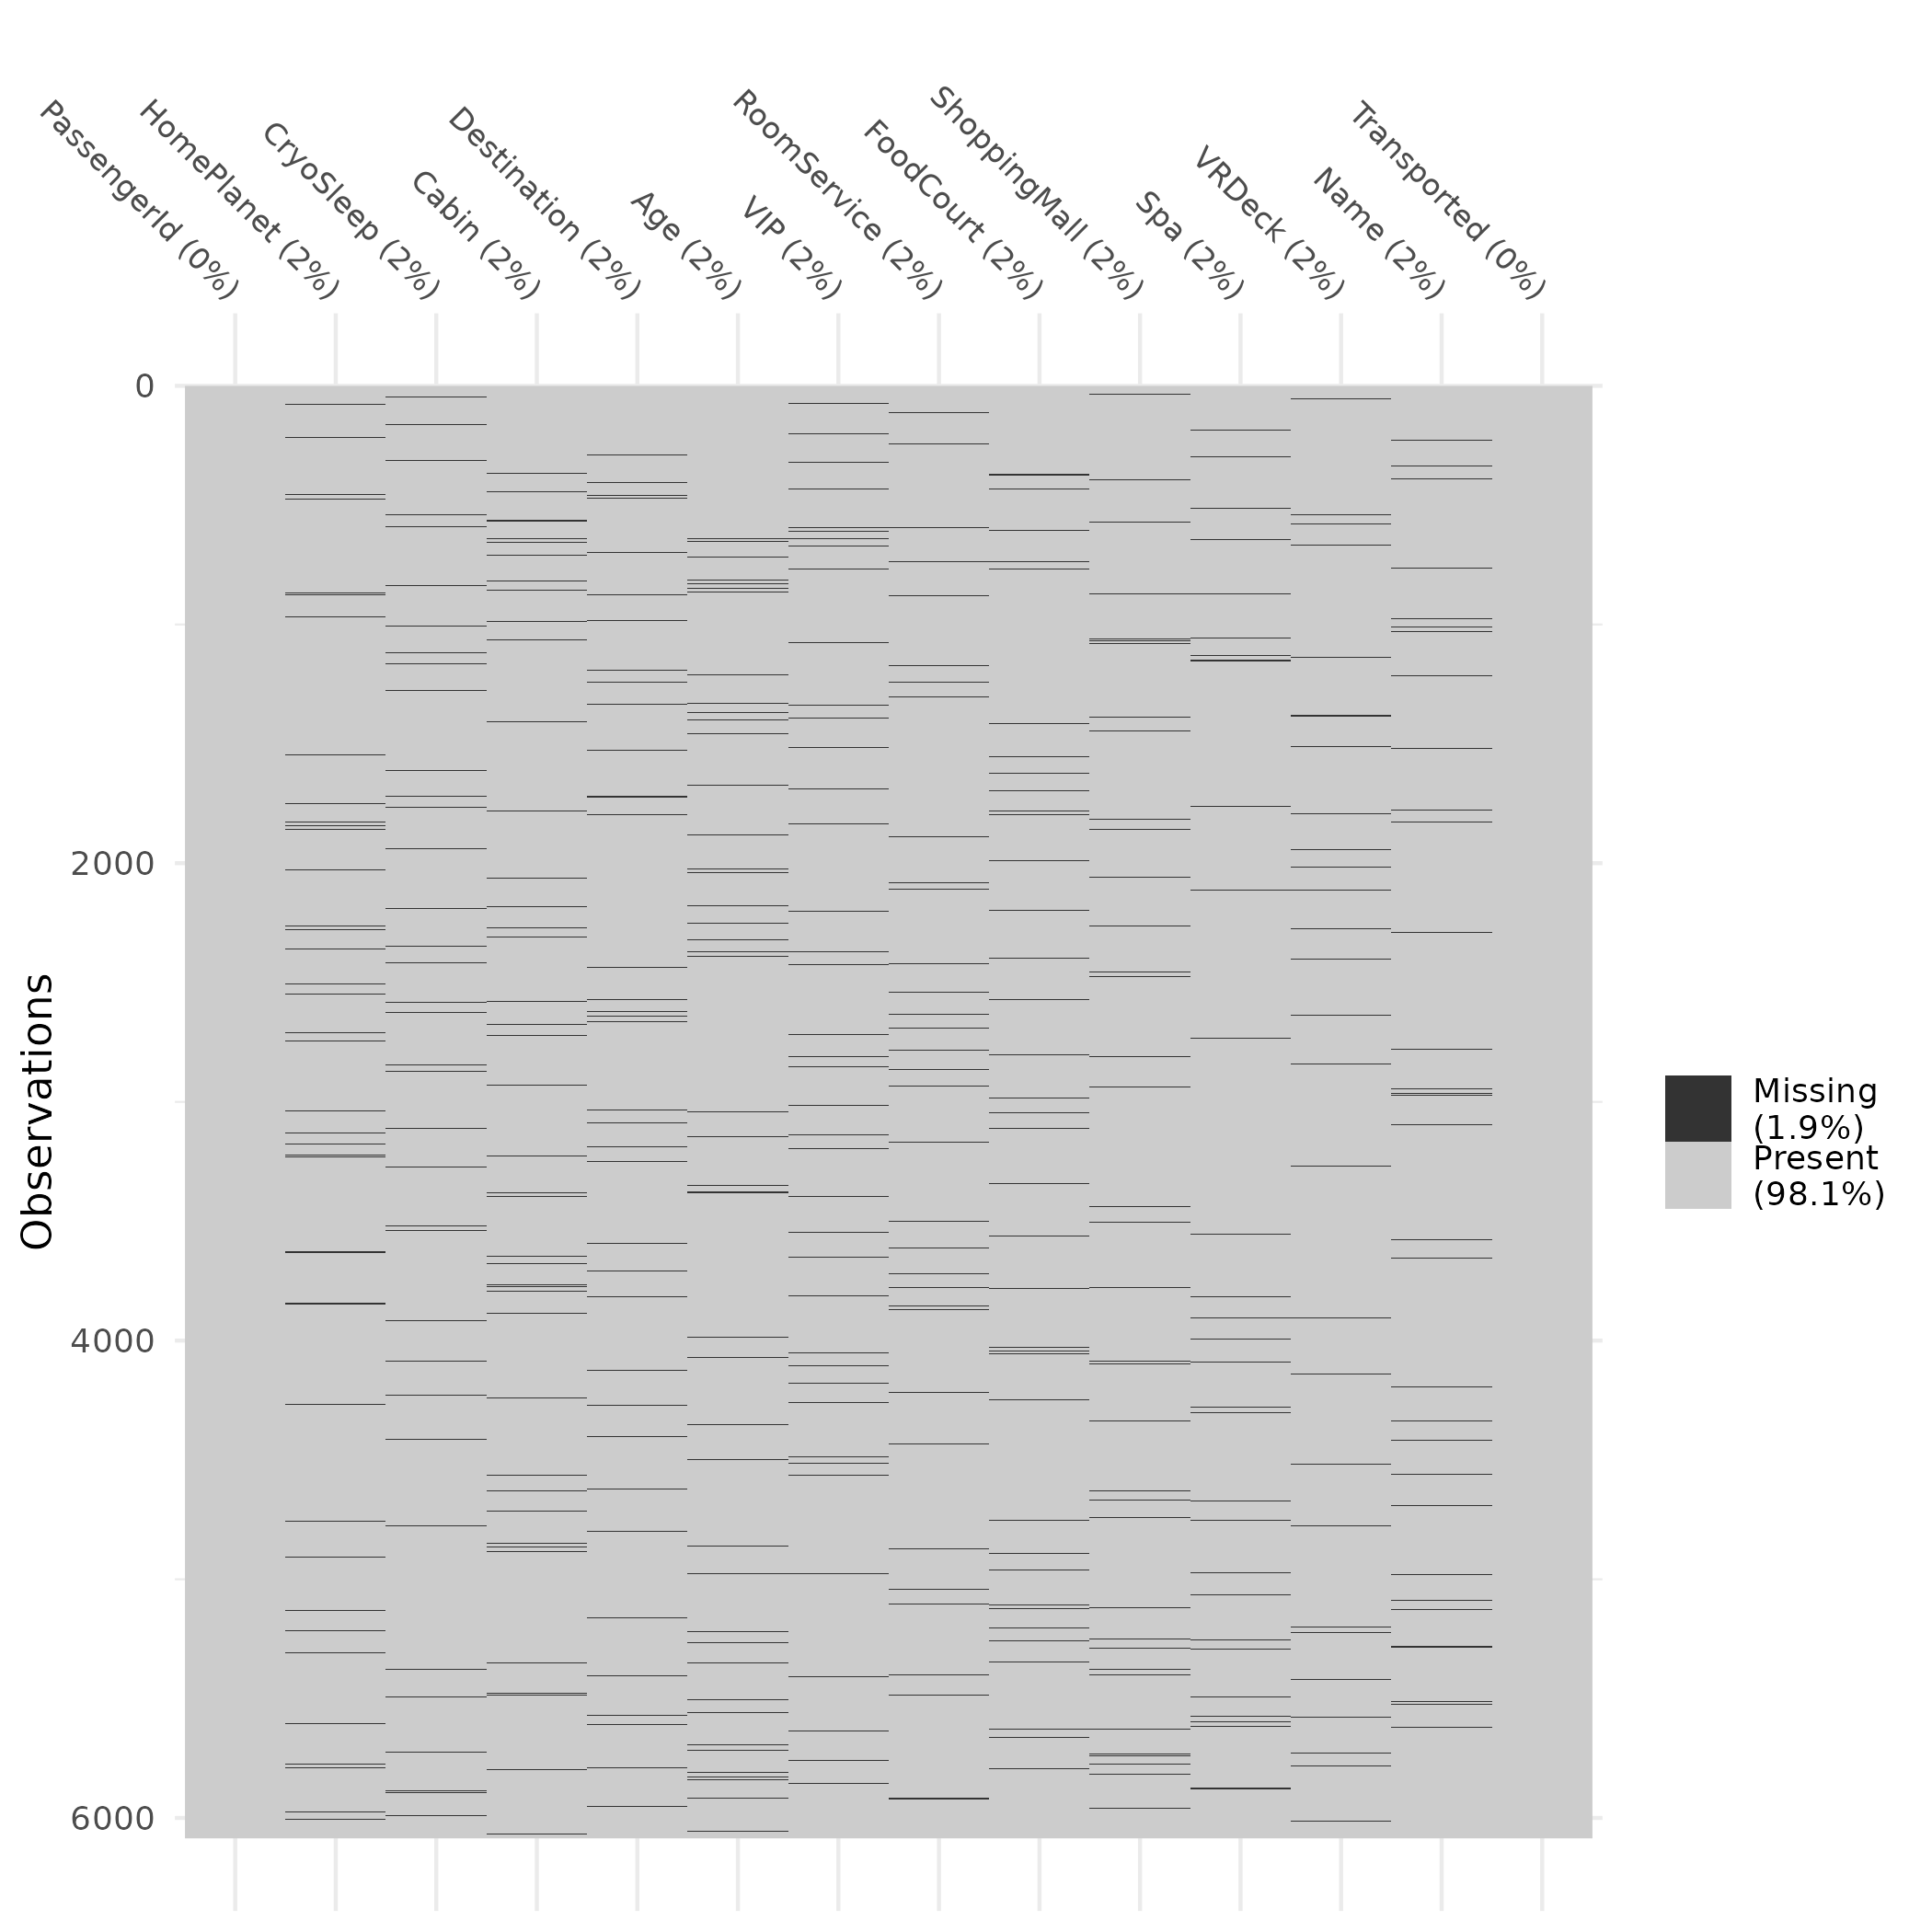
\includegraphics[width=.9\linewidth]{data/visualizations/naniar--missing-values.png}
\end{center}
\subsubsection{Investigando Valores Duplicados}
\label{sec:orgcb88e5f}
Através da contagem, podemos verificar a ausência de valores duplicados.

\begin{verbatim}
# Computar duplicatas no dataset de treinamento
train_duplicates     <- sum(duplicated(train_data) | duplicated(train_data, fromLast = TRUE))
train_duplicates_pct <- round(100 * train_duplicates / nrow(train_data), 2)

# ... e de teste
test_duplicates      <- sum(duplicated(test_data) | duplicated(test_data, fromLast = TRUE))
test_duplicates_pct  <- round(100 * test_duplicates / nrow(test_data), 2)

# produzir dataframe para os dados obtidos
df_duplicates <- data.frame(
  `Treino (abs)` = train_duplicates,
  `Treino (%)`   = train_duplicates_pct,
  `Teste (abs)`  = test_duplicates,
  `Teste (%)`    = test_duplicates_pct,
  check.names    = FALSE
)

cat("Linhas duplicadas (todas as ocorrências):\n")
print(df_duplicates, row.names = FALSE)
\end{verbatim}
\subsection{Análise das \emph{Features}}
\label{sec:orgbb8aa03}
\subsubsection{Separando Colunas Numéricas e Categóricas}
\label{sec:orgd0f5118}
\#+eda-features--separating
\begin{verbatim}
# Extração dos nomes das colunas categóricas e numéricas
column_types <- tibble(
  feature  = names(train_data),
  datatype = map_chr(train_data, ~ class(.)[1]),
  category = case_when(
    map_lgl(train_data, is.numeric) ~ "numerica",

    map_lgl(train_data, ~
                          is.character(.) ||
                          is.factor(.)    ||
                          is.logical(.)
            )                       ~ "categorica",

    map_lgl(train_data, ~
                          inherits(., "Date") ||
                          inherits(., "POSIXct")
            )                       ~ "temporal"
    ),


  missing  = map_int(train_data, ~ sum(is.na(.))),
  unique   = map_int(train_data, n_distinct)
  )

column_types

# Extração dos nomes de colunas por tipo
column_names_by_type <- column_types %>% 
  split(.$category) %>% 
  map(~ .x$feature)
\end{verbatim}

A partir da tabela acima, sabemos que
\begin{itemize}
\item as colunas \texttt{HomePlanet}, \texttt{CryoSleep}, \texttt{Destination} e \texttt{VIP} são verdadeiramente categóricas, apresentando \(3\) ou \(4\) valores;
\item a coluna \texttt{Name} é descrita como categórica porque seu \emph{data type} é \texttt{character} (isto é, \emph{string}).
\end{itemize}
\subsubsection{Análise das Colunas Numéricas}
\label{sec:orgc41321d}
\paragraph{Histogramas}
\label{sec:orgdb3da68}
A fim de investigar \emph{outliers} e a distribuição dos valores numéricos, vamos criar histogramas para todas as \emph{features} desta natureza. Em seguida, vamos usar a biblioteca \texttt{patchwork} para compôr os gráficos em uma visualização única.

\#+eda-features--numerical-histograms
\begin{verbatim}
# Extrair os nomes das colunas numéricas
num_vars <- column_types %>% 
  filter(category == "numerica") %>% 
  pull(feature)

# Criar e salvar cada histograma individualmente usando purrr::map
lista_plots <- map(num_vars, function(col_name) {
  # Nomear o gráfico
  filepath = paste0("data/visualizations/histogram--", col_name, ".png")
  cat("Gerando `", filepath, "`...", sep="")

  # Criar o gráfico dinamicamente
  p <- ggplot(train_data, aes(x = .data[[col_name]])) +
    geom_histogram(fill = "steelblue", color = "white", bins = 20) +
    theme_minimal() +
    labs(
      title = col_name,
      x = col_name,
      y = "Frequência"
    )

  # Salvar o gráfico individual
  ggsave(
    filename = filepath,
    plot     = p
  )

  return(p) # Retorna o objeto do gráfico para a lista
})

# Compôr os histogramas com patchwork
composition <- wrap_plots(lista_plots, ncol = 3) + 
  plot_annotation(
    title = "Histogramas das Features Numéricas",
    theme = theme(plot.title = element_text(size = 16, face = "bold", hjust = 0.5))
  )

cat("Gerando composição de gráficos...")
ggsave(filename=paste0(PATH_VIS, "histogram--composition.png"), plot=composition)
\end{verbatim}

\begin{center}
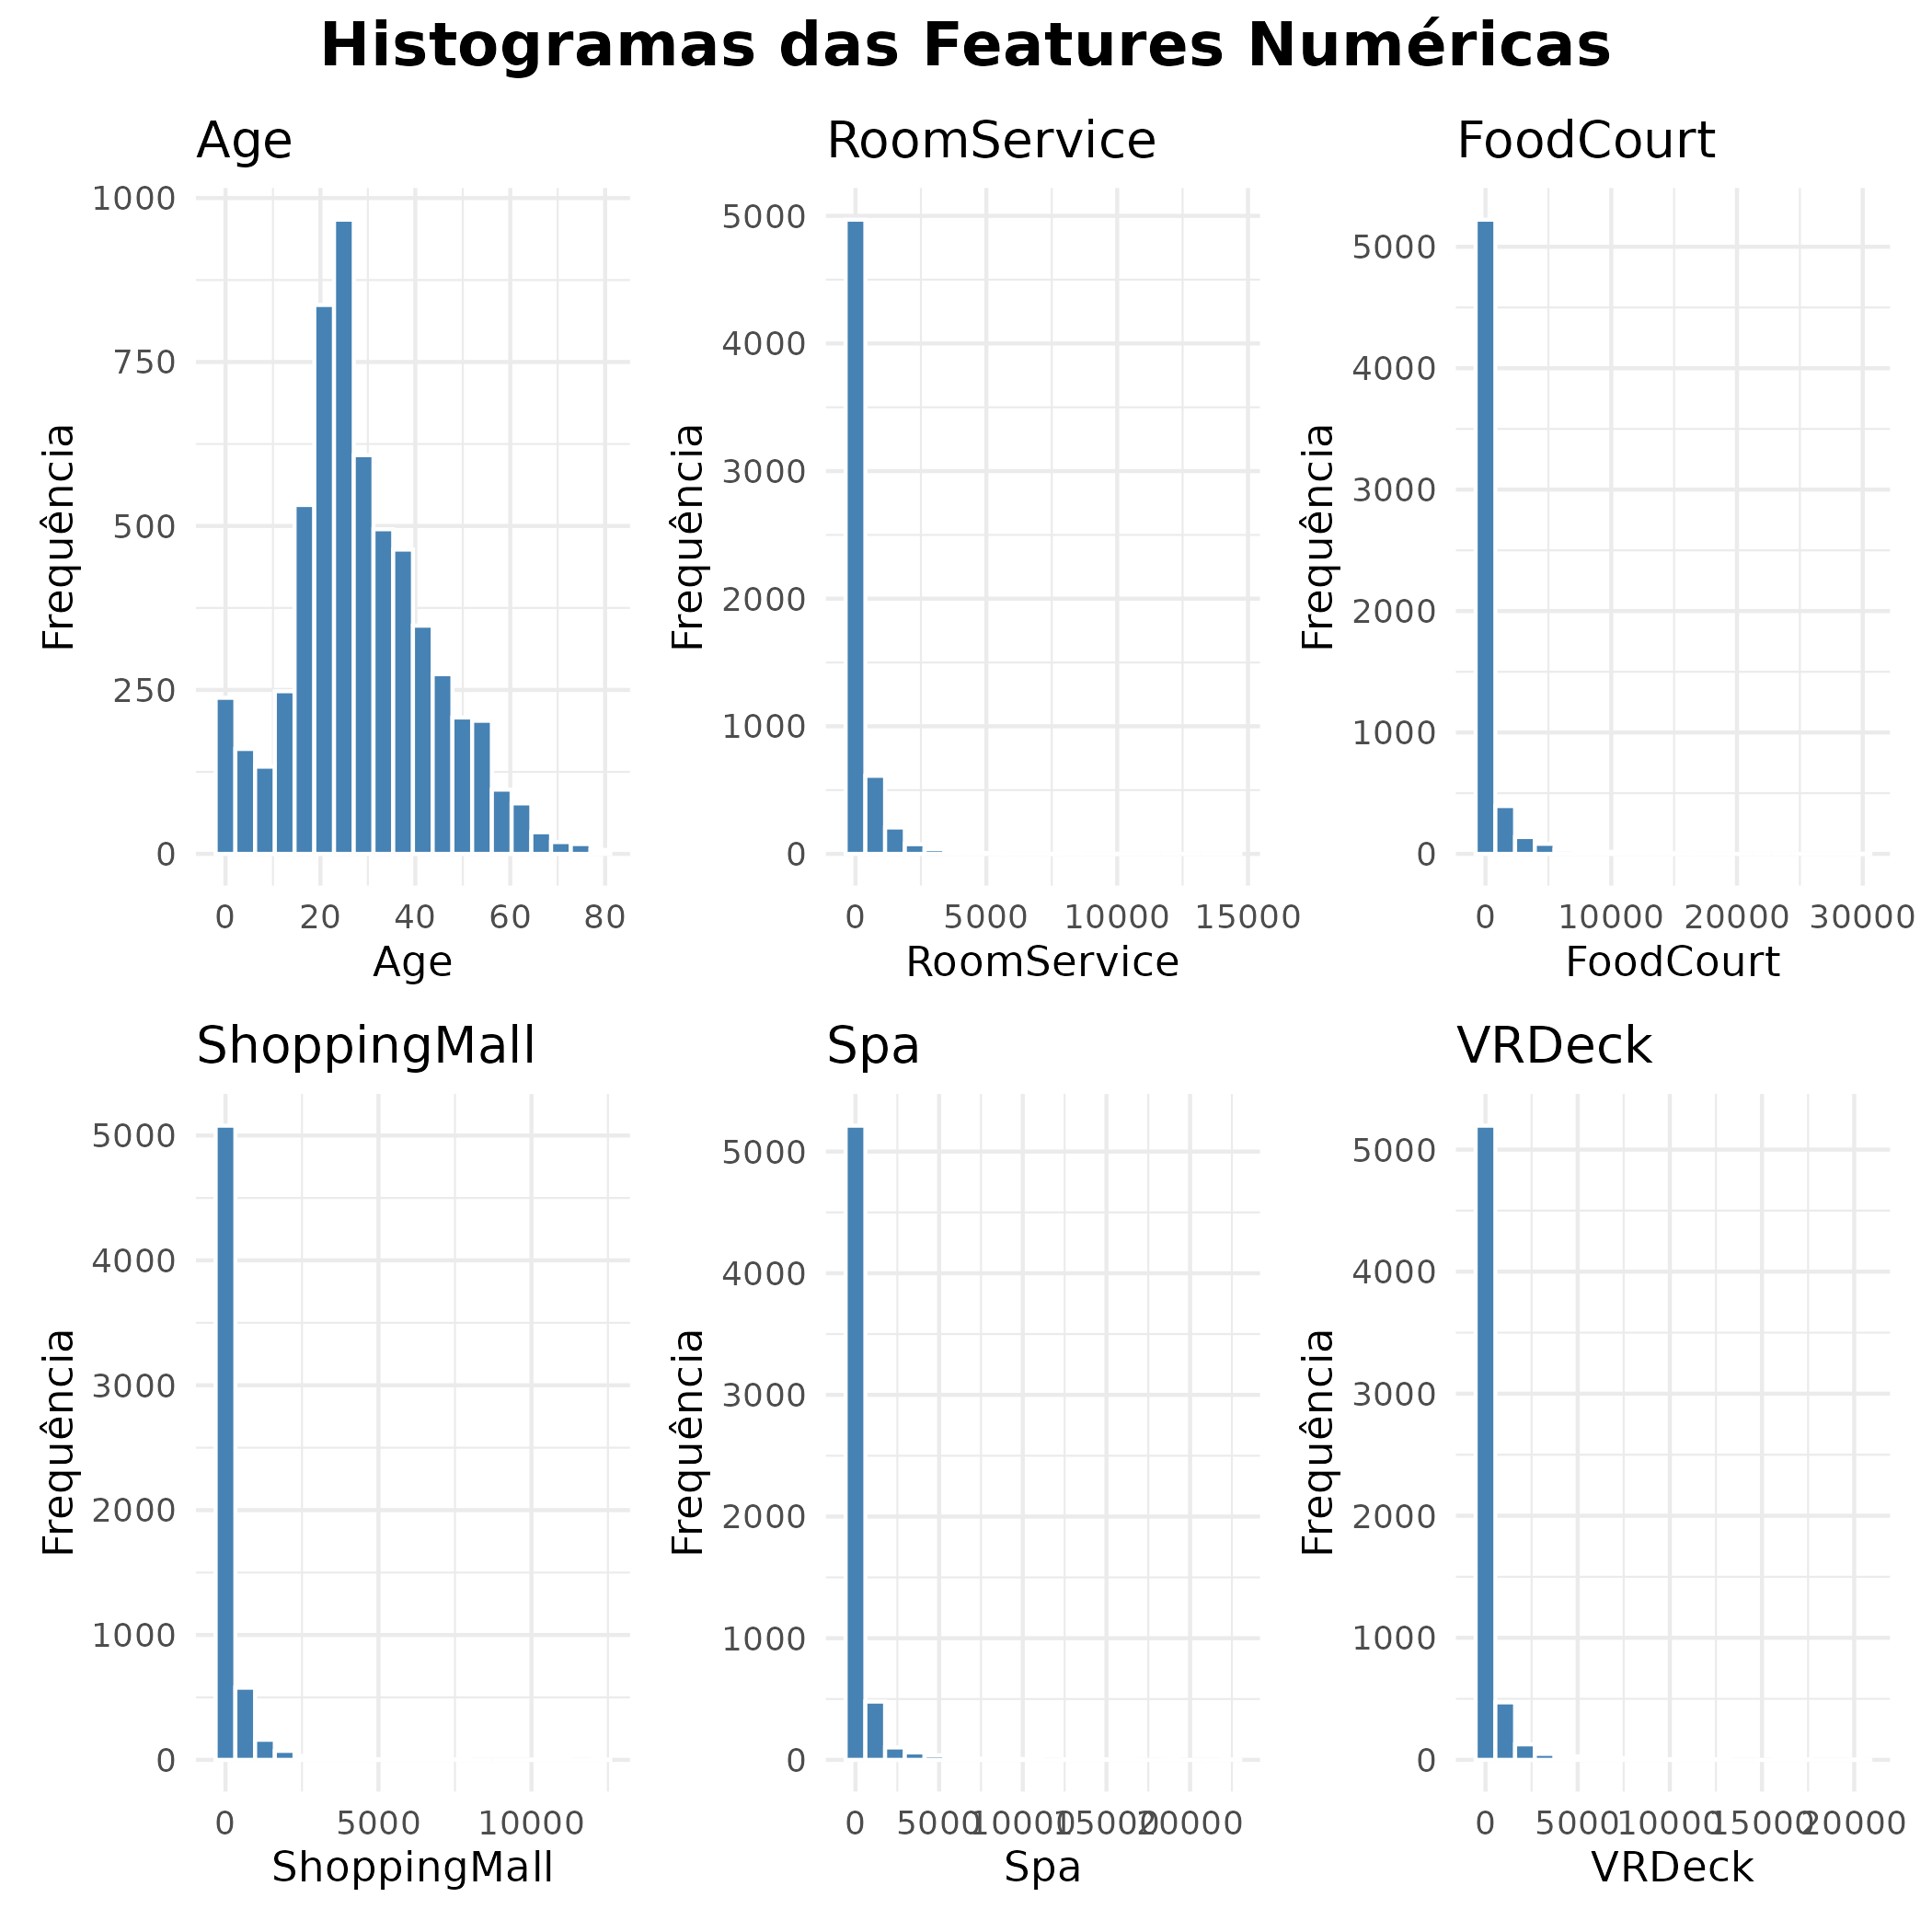
\includegraphics[width=.9\linewidth]{data/visualizations/histogram--composition.png}
\end{center}
\paragraph{\emph{Boxplots} relacionando \texttt{Transported}}
\label{sec:org586ce23}
\#+eda-features--numerical-boxplots
\begin{verbatim}
lista_plots <- map(num_vars, function(col_name) {

  # Converter para numérico e remover NAs temporariamente para o cálculo do boxplot
  dados_plot <- train_data[!is.na(train_data[[col_name]]), ]
  dados_plot[[col_name]] <- as.numeric(dados_plot[[col_name]])

  # Criar o gráfico garantindo eixos explícitos
  p <- ggplot(dados_plot,
              aes(x = factor(Transported), y = .data[[col_name]], fill = factor(Transported))) +
              # outlier.shape = NA esconde os pontos gigantes que esmagam o gráfico
              geom_boxplot(outlier.shape = NA, width = 0.6) + 
              # Ajusta o zoom para focar onde a maioria dos dados está (95% centrais)
              coord_cartesian(ylim = quantile(dados_plot[[col_name]], c(0, 0.95), na.rm = TRUE)) +
              labs(
                title = paste0("Transported vs. ", col_name),
                x = "Transportado",
                y = "Valor"
              ) +
              theme_minimal(base_size = 9) + # Diminui o texto para caber no grid
              theme(legend.position = "none") # Remove legendas repetidas


  return(p)
})

# Compôr o grid com escalas livres para evitar distorção
composition <- wrap_plots(lista_plots, ncol = 2) + 
  plot_layout(guides = "collect") + # Junta as legendas se houver
  plot_annotation(
    title = "Boxplots: Features Numéricas vs. Transported",
    theme = theme(plot.title = element_text(size = 12, face = "bold", hjust = 0.5))
  )

cat("Gerando composição de gráficos...")
ggsave(filename=paste0(PATH_VIS, "boxplot--composition.png"), plot=composition)
\end{verbatim}


\begin{center}
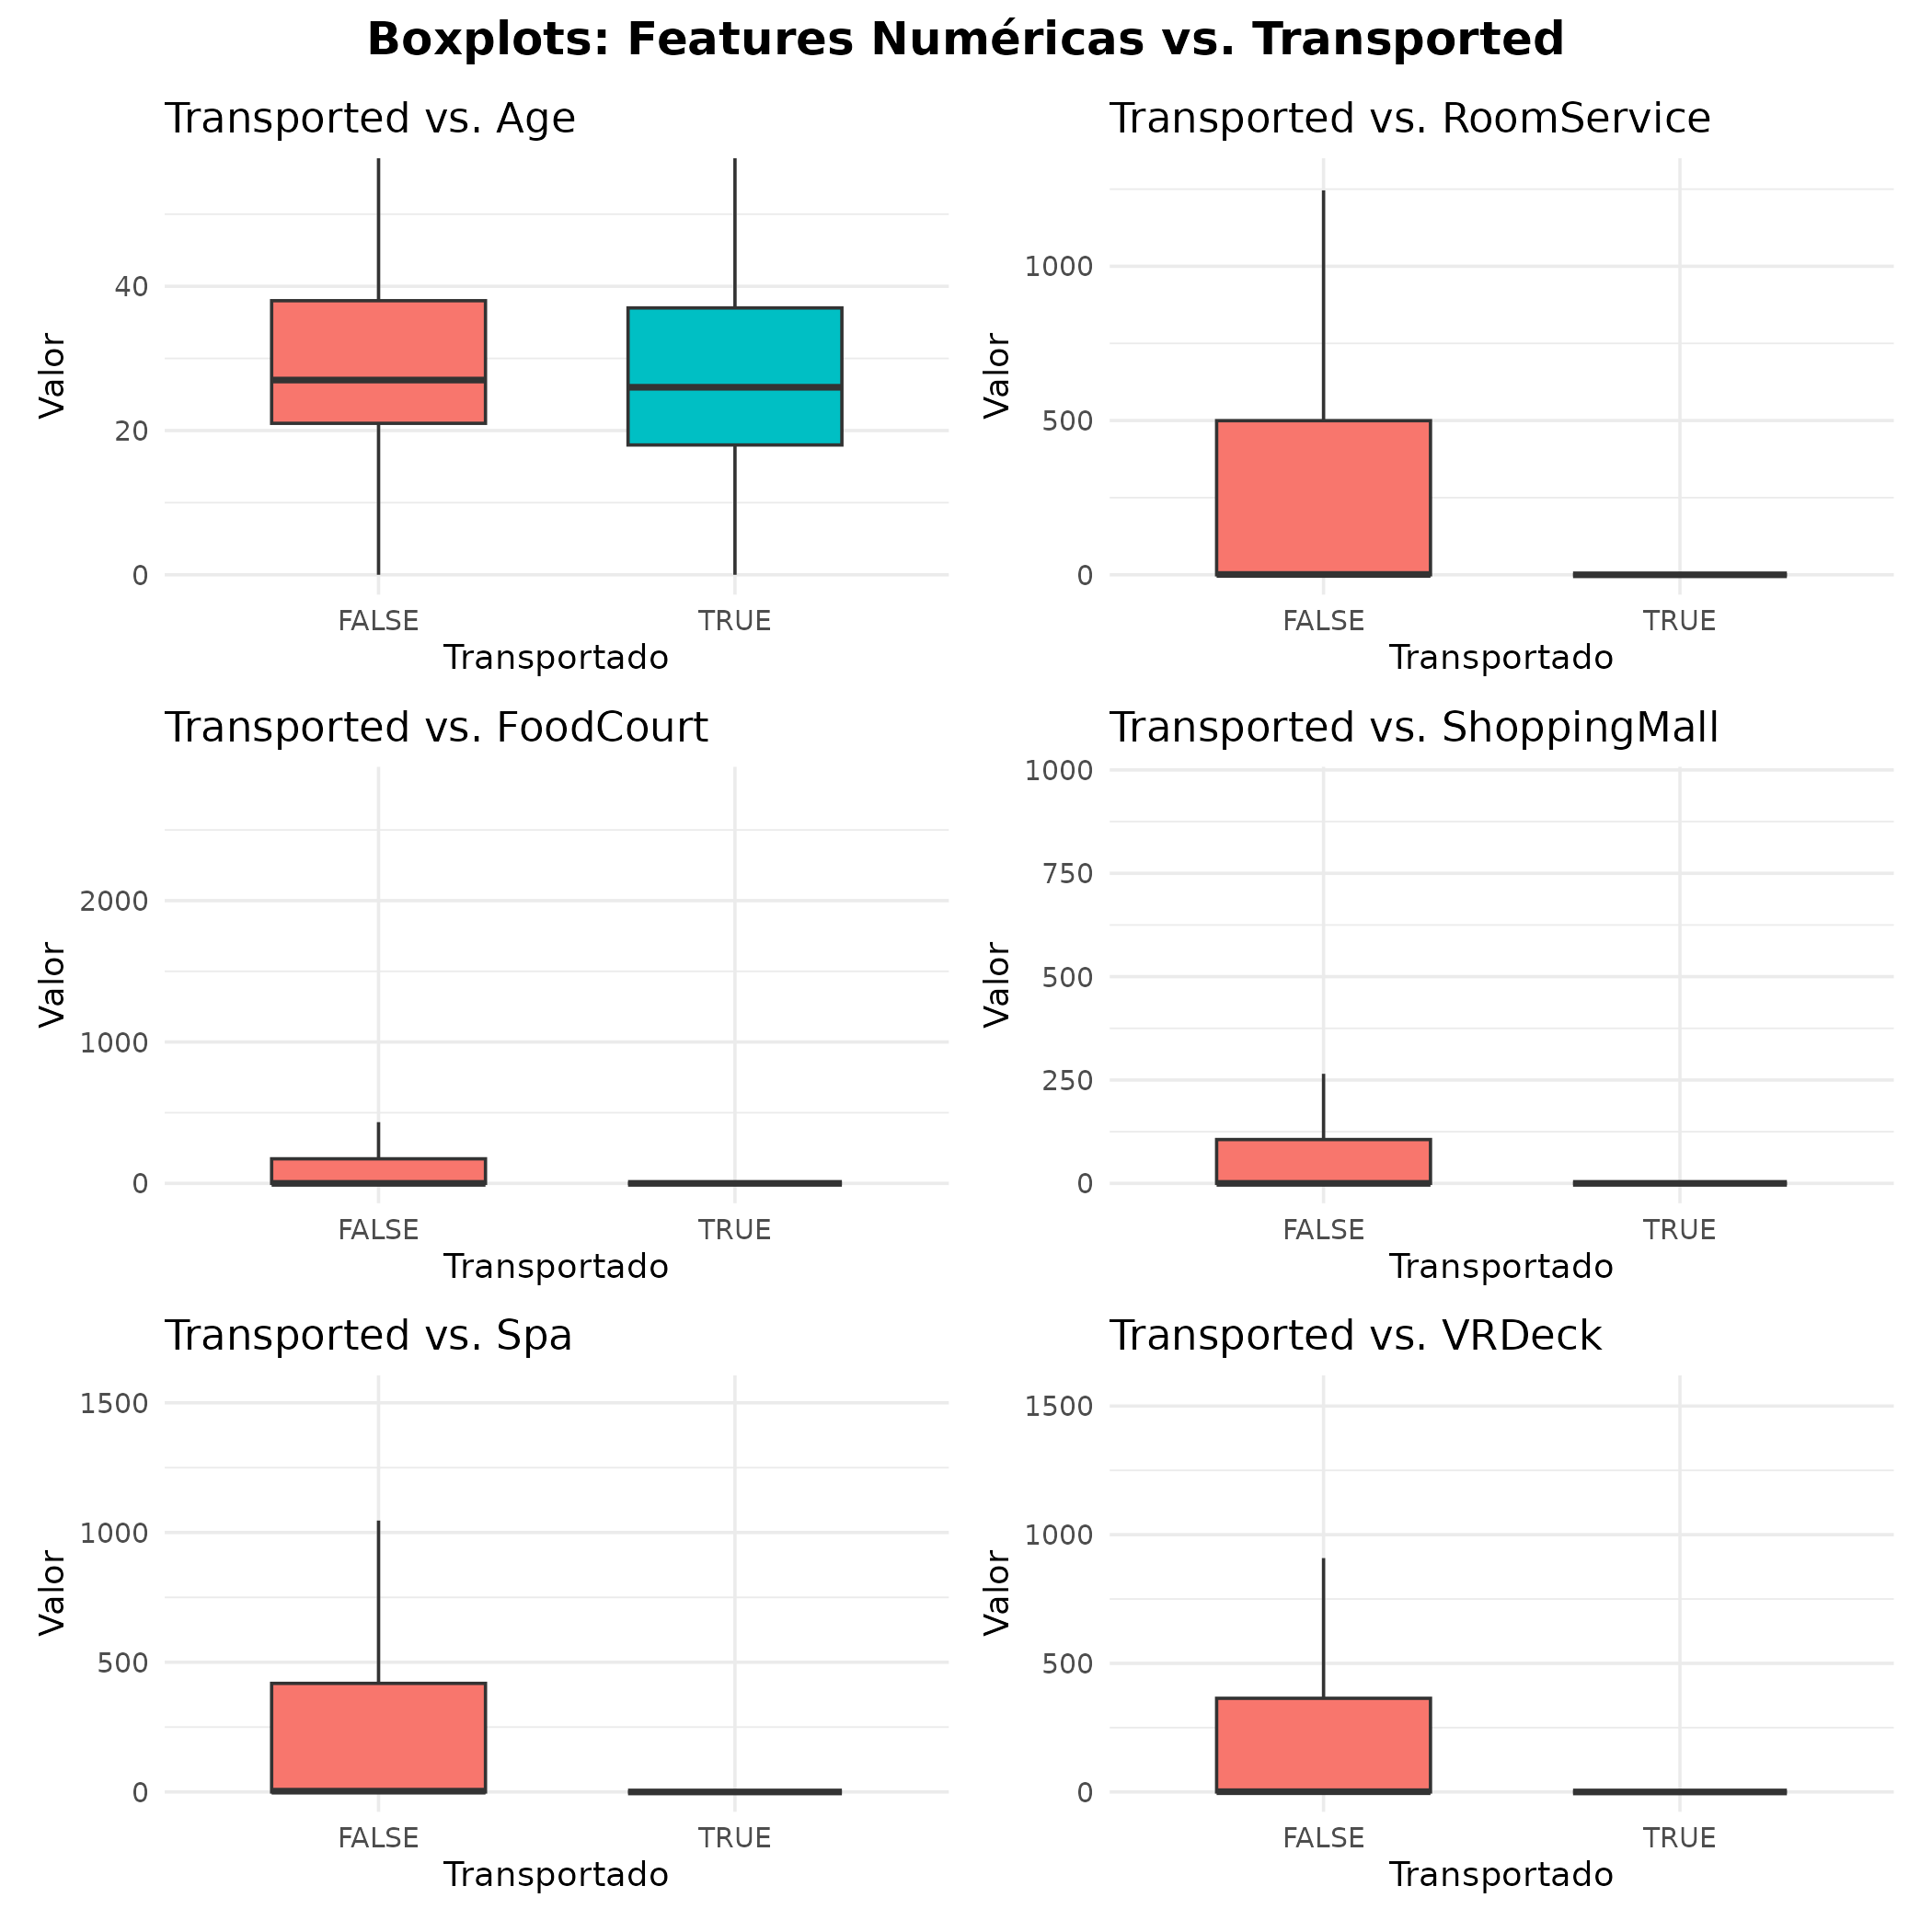
\includegraphics[width=.9\linewidth]{data/visualizations/boxplot--composition.png}
\end{center}
\paragraph{Distruições com Gráfico de Violino}
\label{sec:org30b0413}
\#+eda-features--numerical-violins
\begin{verbatim}
lista_plots <- map(num_vars, function(col_name) {

  dados_plot <- train_data[!is.na(train_data[[col_name]]), ]
  dados_plot[[col_name]] <- as.numeric(dados_plot[[col_name]])

  p <- ggplot(dados_plot,
              aes(x = factor(Transported), y = .data[[col_name]], fill = factor(Transported))) +
              # 1. Gráfico de violino mostra a distribuição/concentração mesmo se for zero
              geom_violin(alpha = 0.4, color = NA, scale = "width") +
              # 2. Adiciona os pontos reais levemente espalhados para ver a amostragem
              geom_jitter(aes(color = factor(Transported)), alpha = 0.1, width = 0.2) +
              # 3. Escala logarítmica + 1 para lidar com valores zero sem quebrar o gráfico
              scale_y_log10(labels = scales::label_comma()) +
              labs(
                title = paste0("vs. ", col_name),
                x = "Transportado",
                y = paste0(col_name, " (Log10)")
              ) +
              theme_minimal(base_size = 9) +
              theme(legend.position = "none")

  return(p)
})

# Recompor o layout com patchwork
composition <- wrap_plots(lista_plots, ncol = 2) + 
  plot_annotation(
    title = "Distribuição: Features Numéricas vs. Transported",
    theme = theme(plot.title = element_text(size = 12, face = "bold", hjust = 0.5))
  )

ggsave(filename="data/visualizations/distribution-violins.png", plot=composition)
\end{verbatim}

\begin{center}
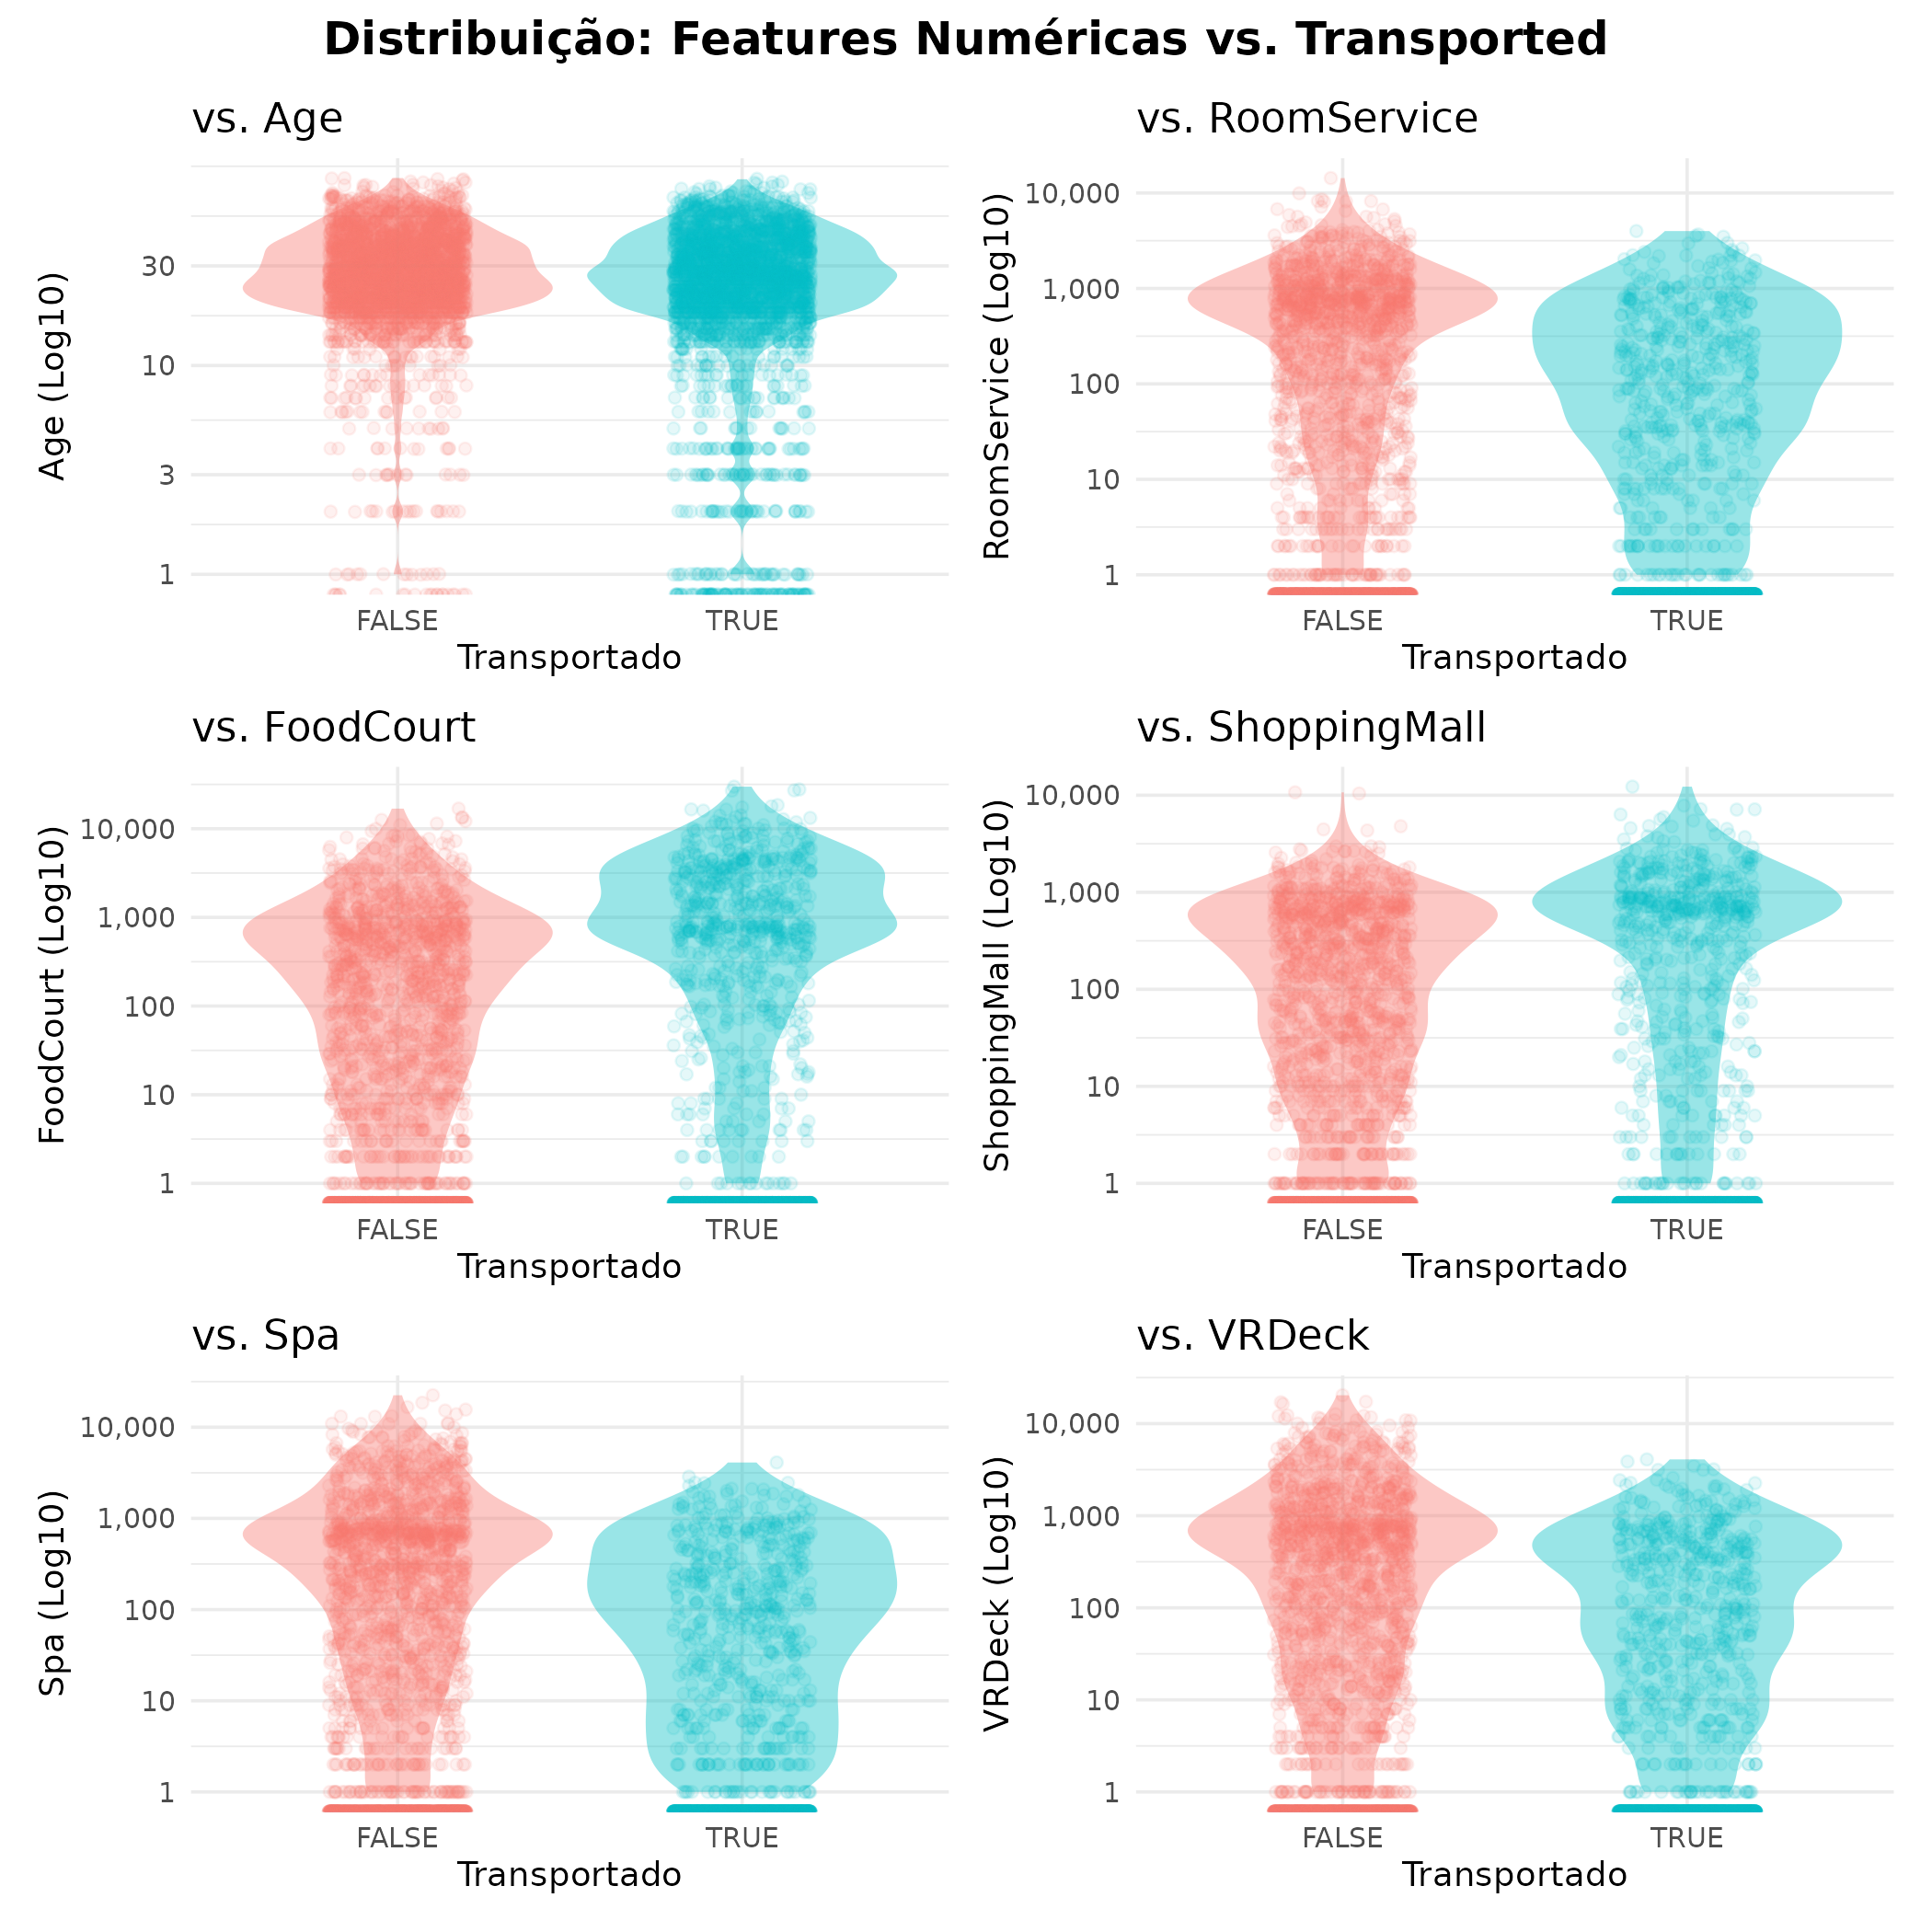
\includegraphics[width=.9\linewidth]{data/visualizations/distribution-violins.png}
\end{center}
\paragraph{Boxplots para identificar outliers}
\label{sec:org2022b2b}
\#+eda-features--identifying-outliers
\begin{verbatim}
dist <- train_data %>%
  select(Age, RoomService, FoodCourt, ShoppingMall, Spa, VRDeck) %>%
  pivot_longer(everything(), names_to = "variavel", values_to = "valor") %>%
  filter(!is.na(valor)) %>%          # remove NAs
  ggplot(aes(x = variavel, y = valor + 1)) +  # +1 permite log de zero
  geom_boxplot() +
  scale_y_log10() +
  labs(y = "valor + 1 (escala log10)", title = "Distribuição das variáveis numéricas")

print("Gerando boxplots para identificação de outliers...")
ggsave(filename="data/visualizations/distribution-outliers.png", plot=dist)
\end{verbatim}

\begin{center}
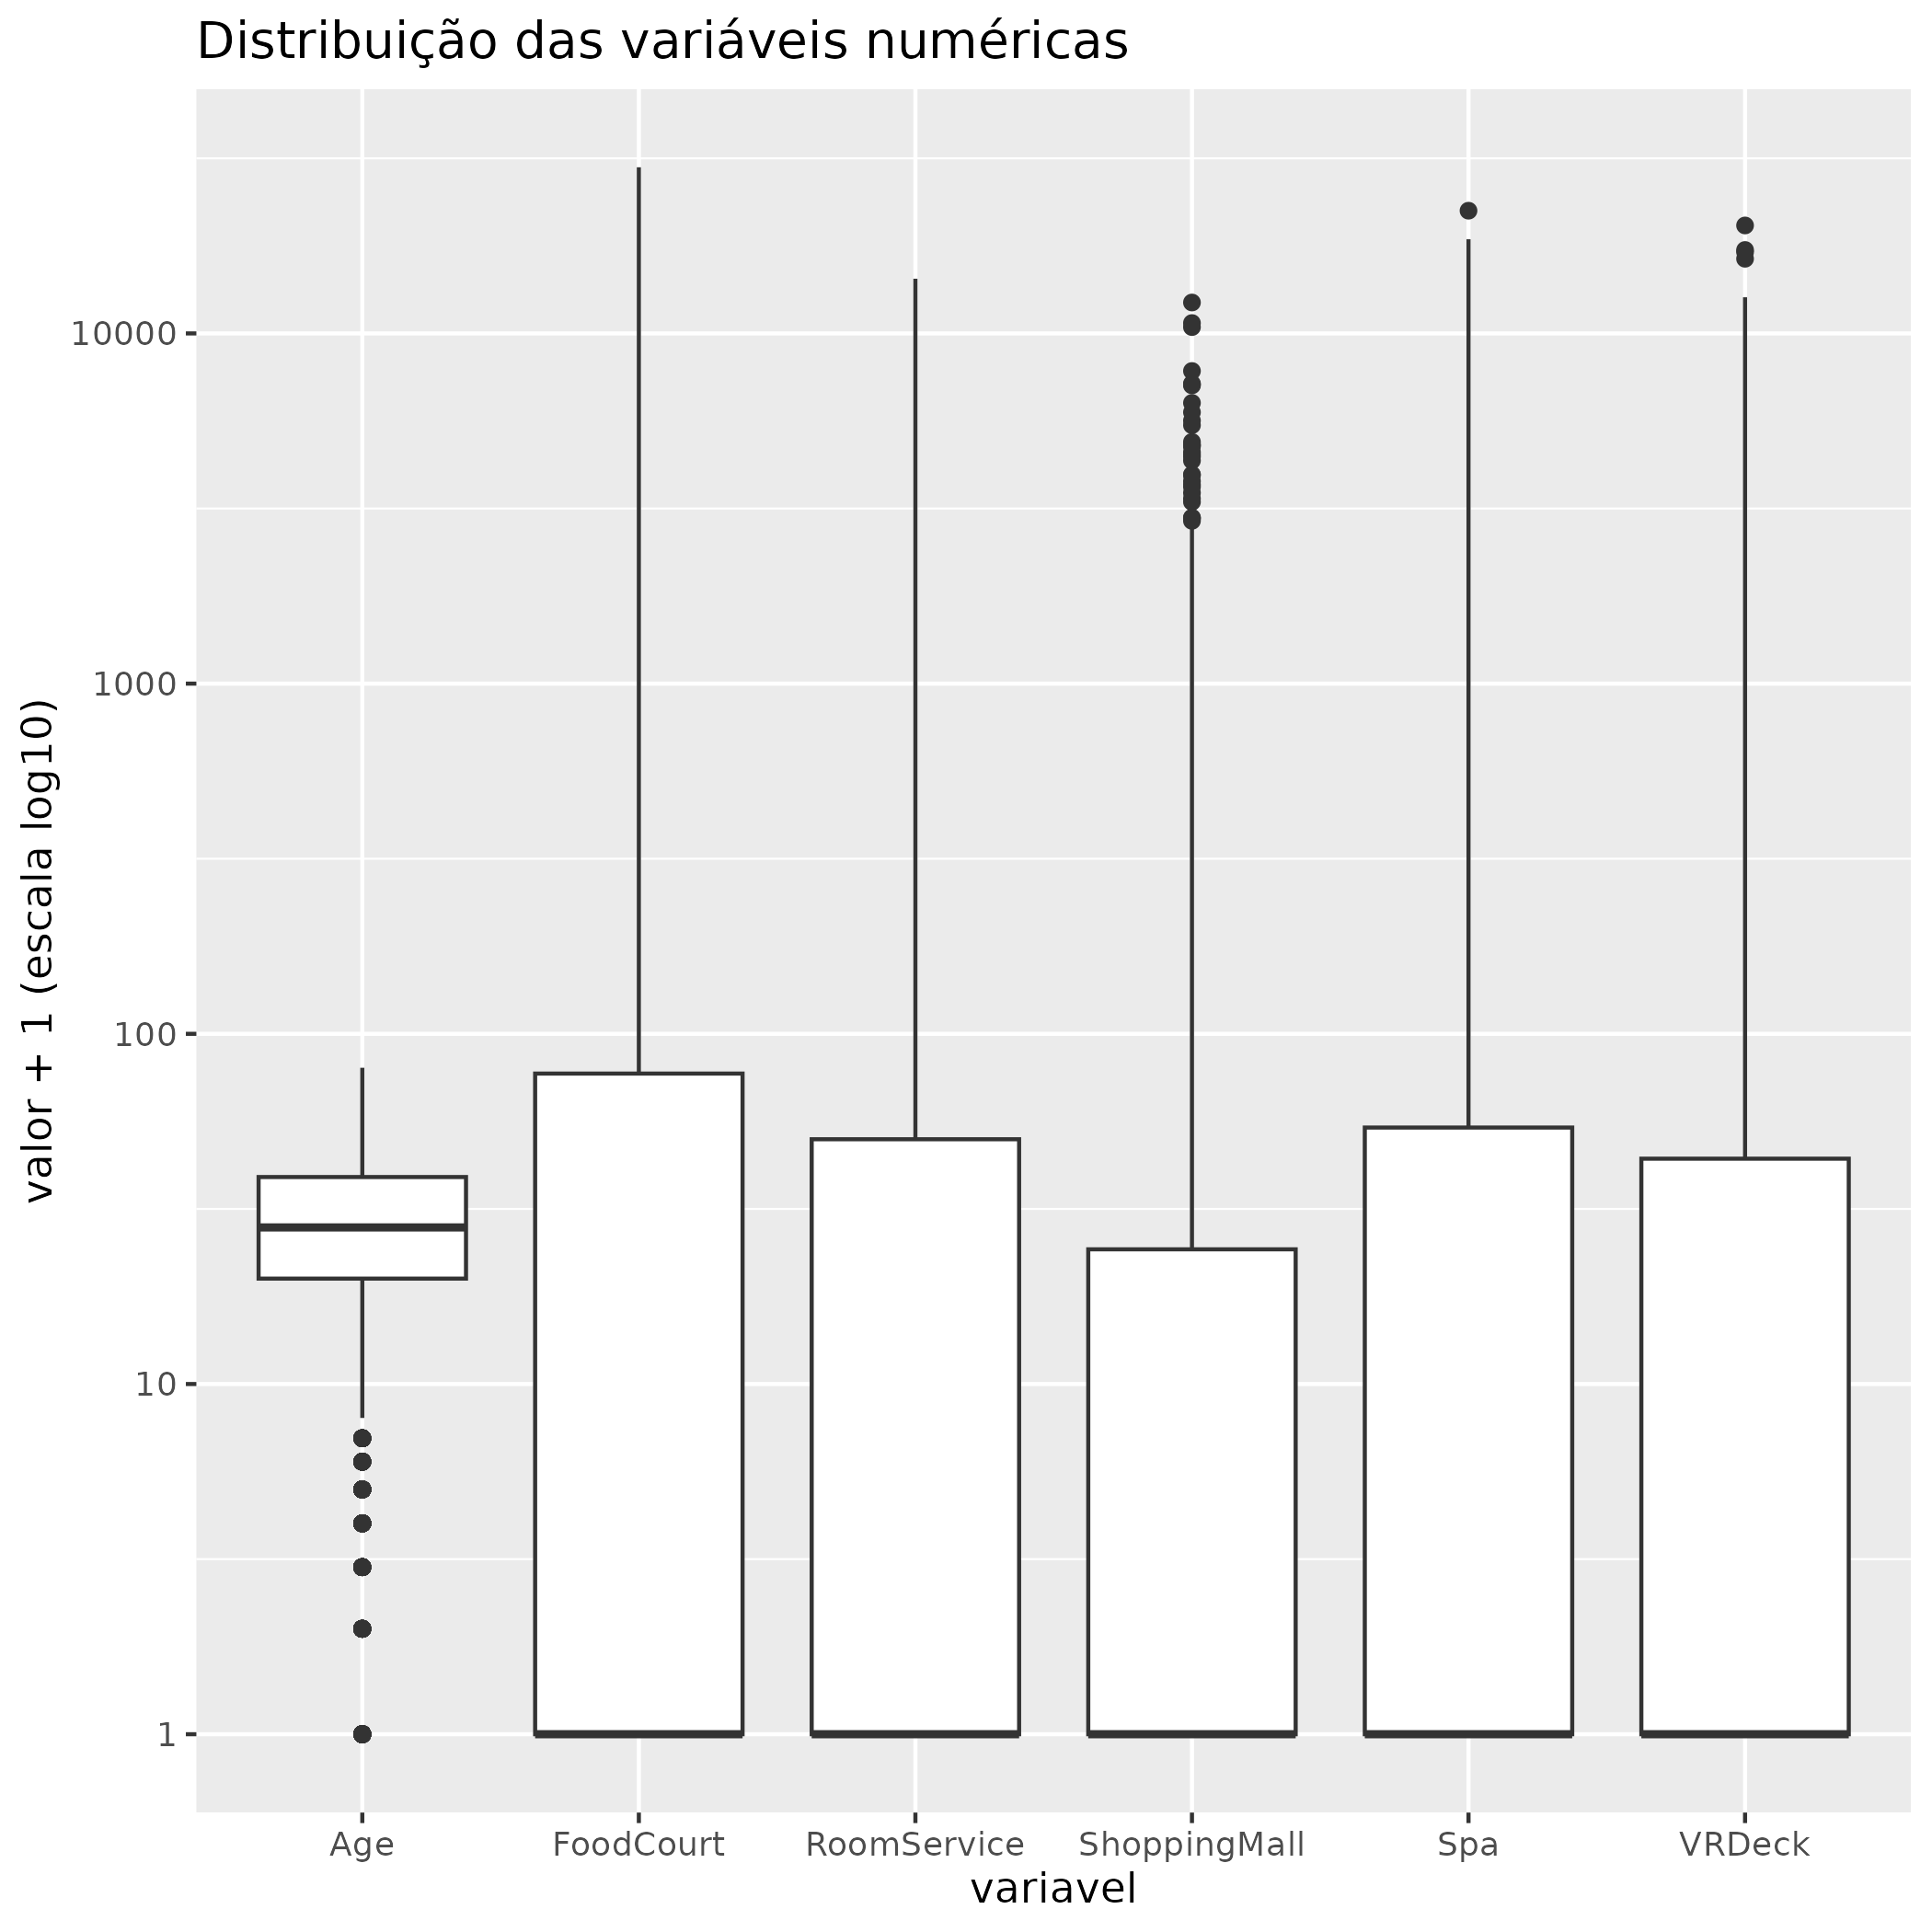
\includegraphics[width=.9\linewidth]{data/visualizations/distribution-outliers.png}
\end{center}
\paragraph{Densidade de \texttt{Age} estratificada por \texttt{Transported}}
\label{sec:org3d30a3a}
\begin{verbatim}
density <- train_data %>%
  filter(!is.na(Age)) %>%
  ggplot(aes(x = Age, fill = Transported)) +
  geom_density(alpha = 0.5, na.rm = TRUE) +
  theme_minimal()

print("Gerando gráfico de densidade entre Age e Transported...")
ggsave(filename="data/visualizations/density--Age-Transported.png", plot=density)
\end{verbatim}

\begin{center}
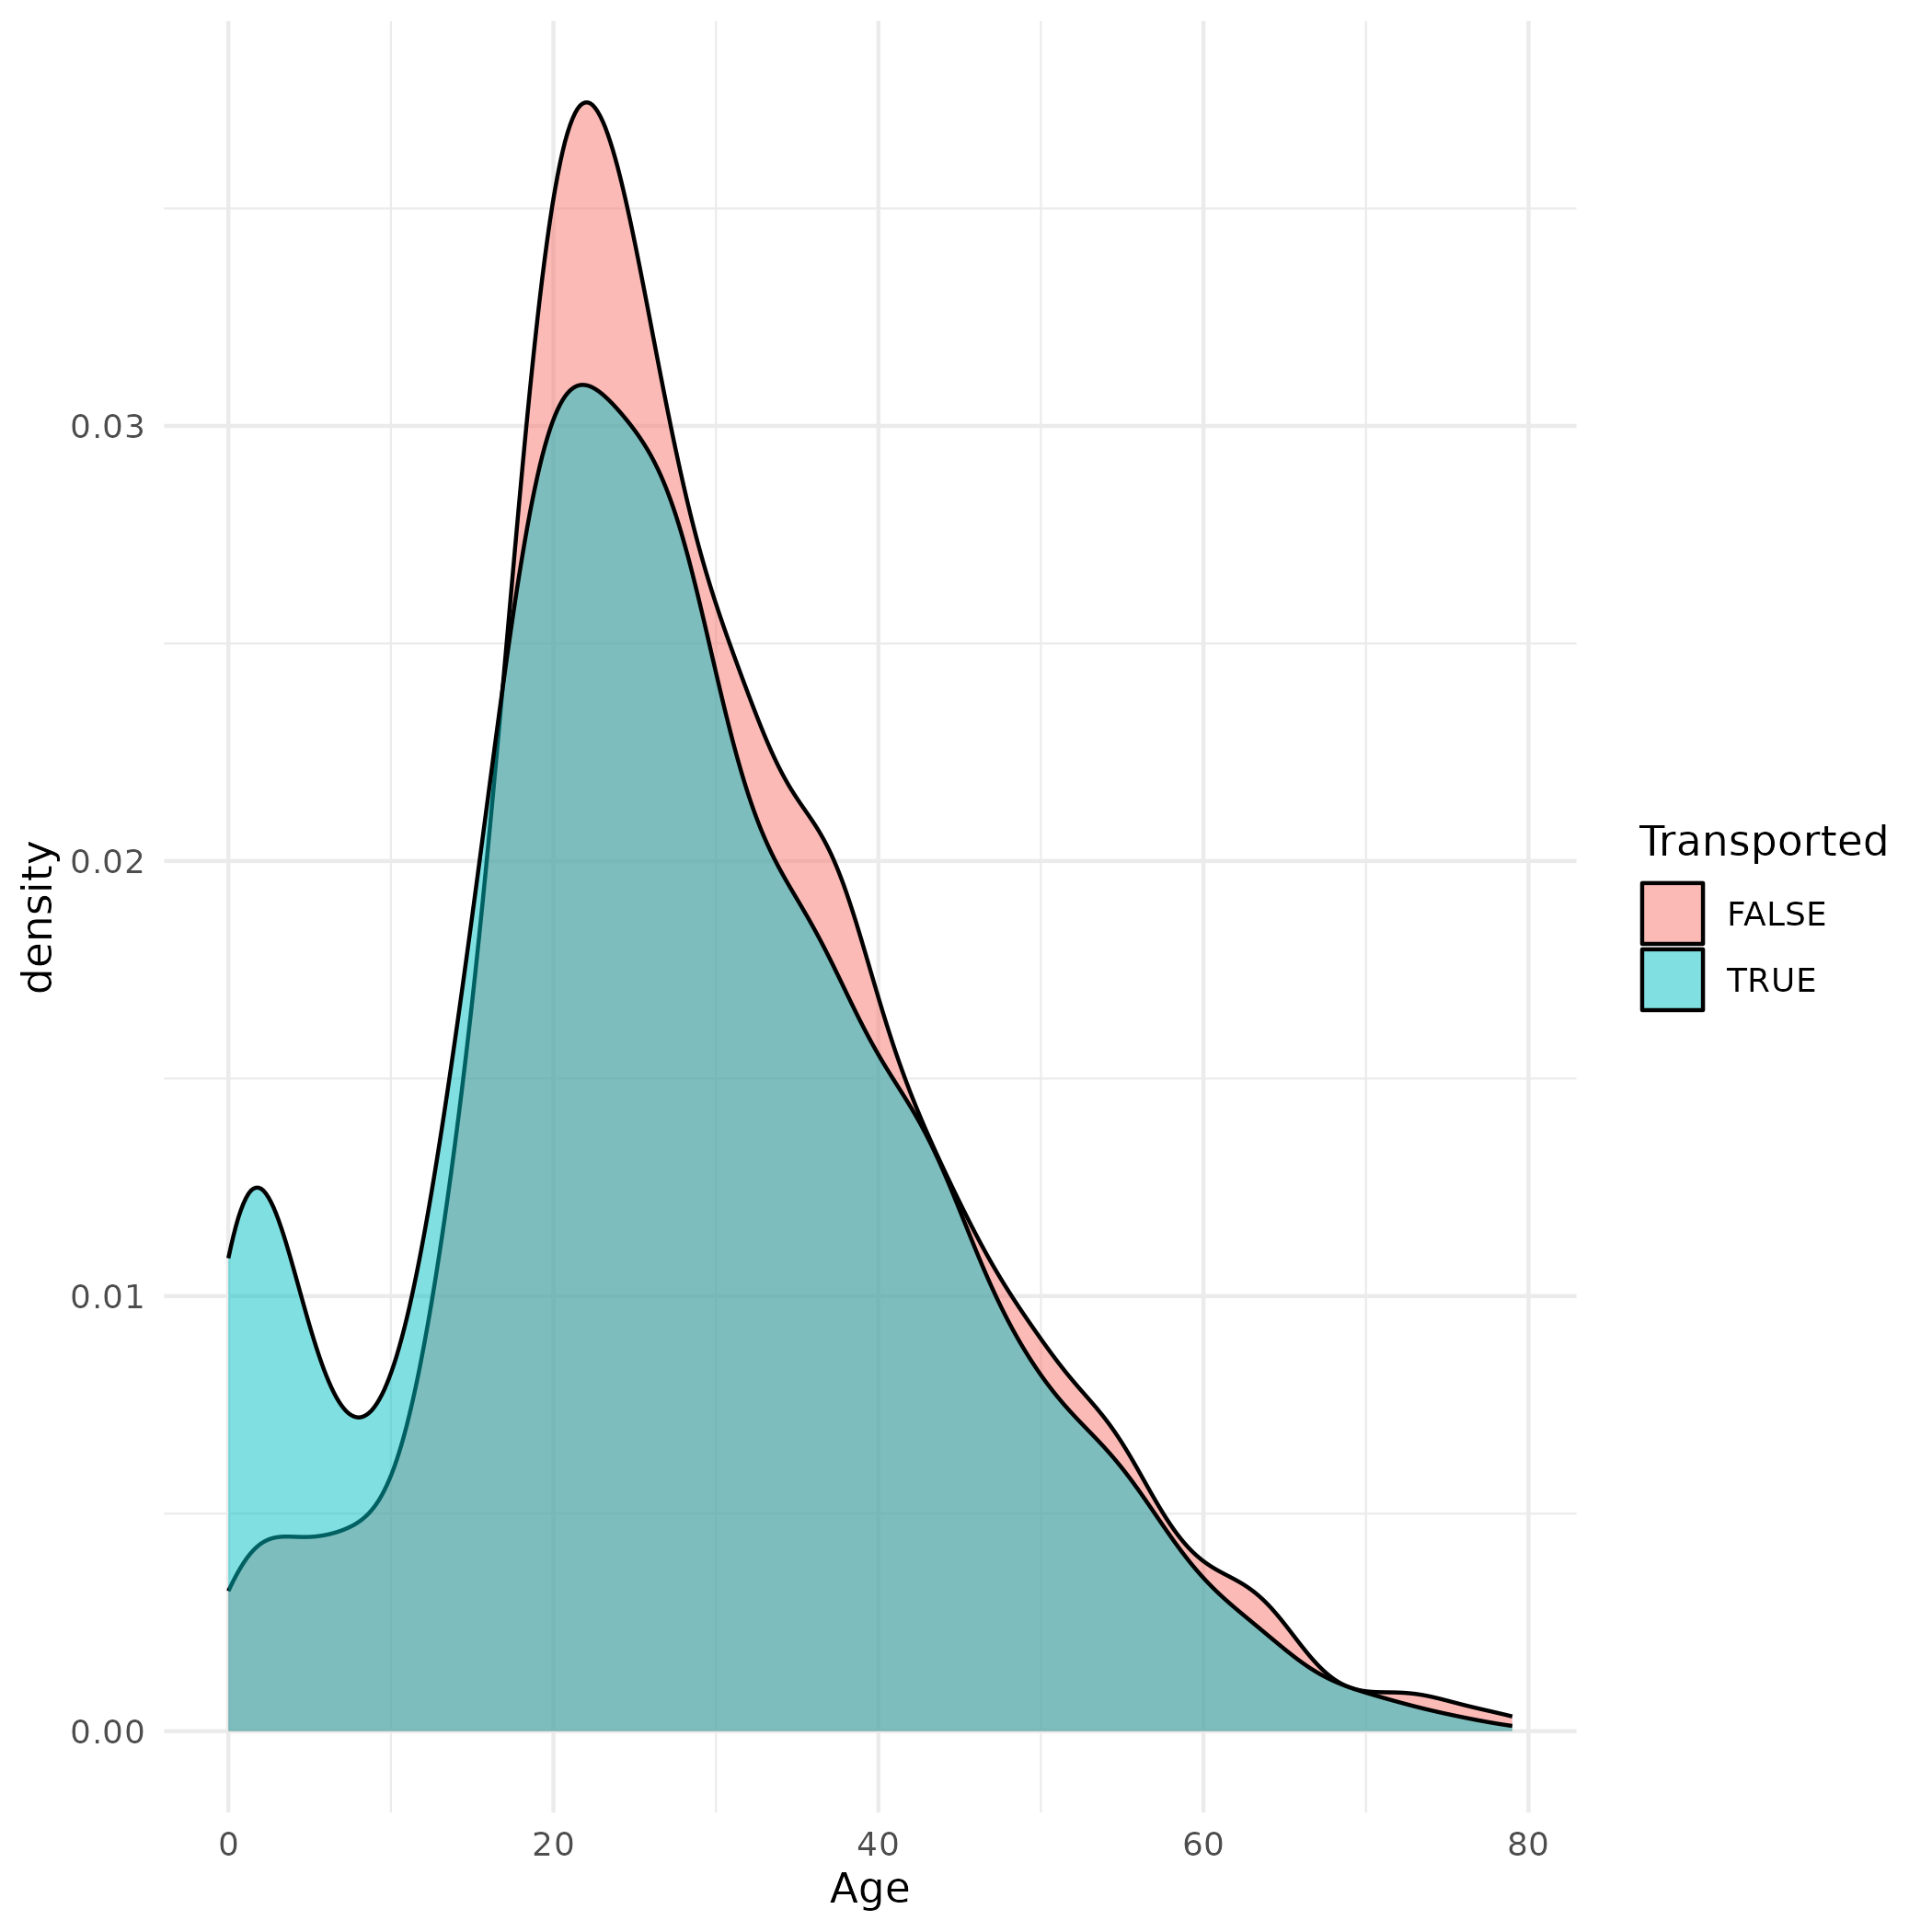
\includegraphics[width=.9\linewidth]{data/visualizations/density--Age-Transported.png}
\end{center}
\subsubsection{Análise Univariada para Variáveis Categóricas}
\label{sec:orgcc91e04}
Gráfico de barras para \texttt{HomePlanet}, \texttt{CryoSleep}, \texttt{Destination} e \texttt{VIP}.

\begin{verbatim}
dist_cat <- train_data %>%
  select(HomePlanet, CryoSleep, Destination, VIP, Transported) %>%
  mutate(
    CryoSleep = as.character(CryoSleep),
    VIP = as.character(VIP)
  ) %>%
  pivot_longer(-Transported, names_to = "variavel", values_to = "categoria") %>%
  filter(!is.na(categoria)) %>%
  ggplot(aes(x = categoria, fill = Transported)) +
  geom_bar(position = "fill") +
  facet_wrap(~variavel, scales = "free_x") +
  theme_minimal() +
  labs(y = "Proporção", title = "Relação entre variáveis categóricas e Transported")

print("Gerando barplots para features categóricas...")
ggsave(filename="data/visualizations/barplots--Transported-vs-Categorical_Features.png",
       plot = dist_cat)
\end{verbatim}

\begin{center}
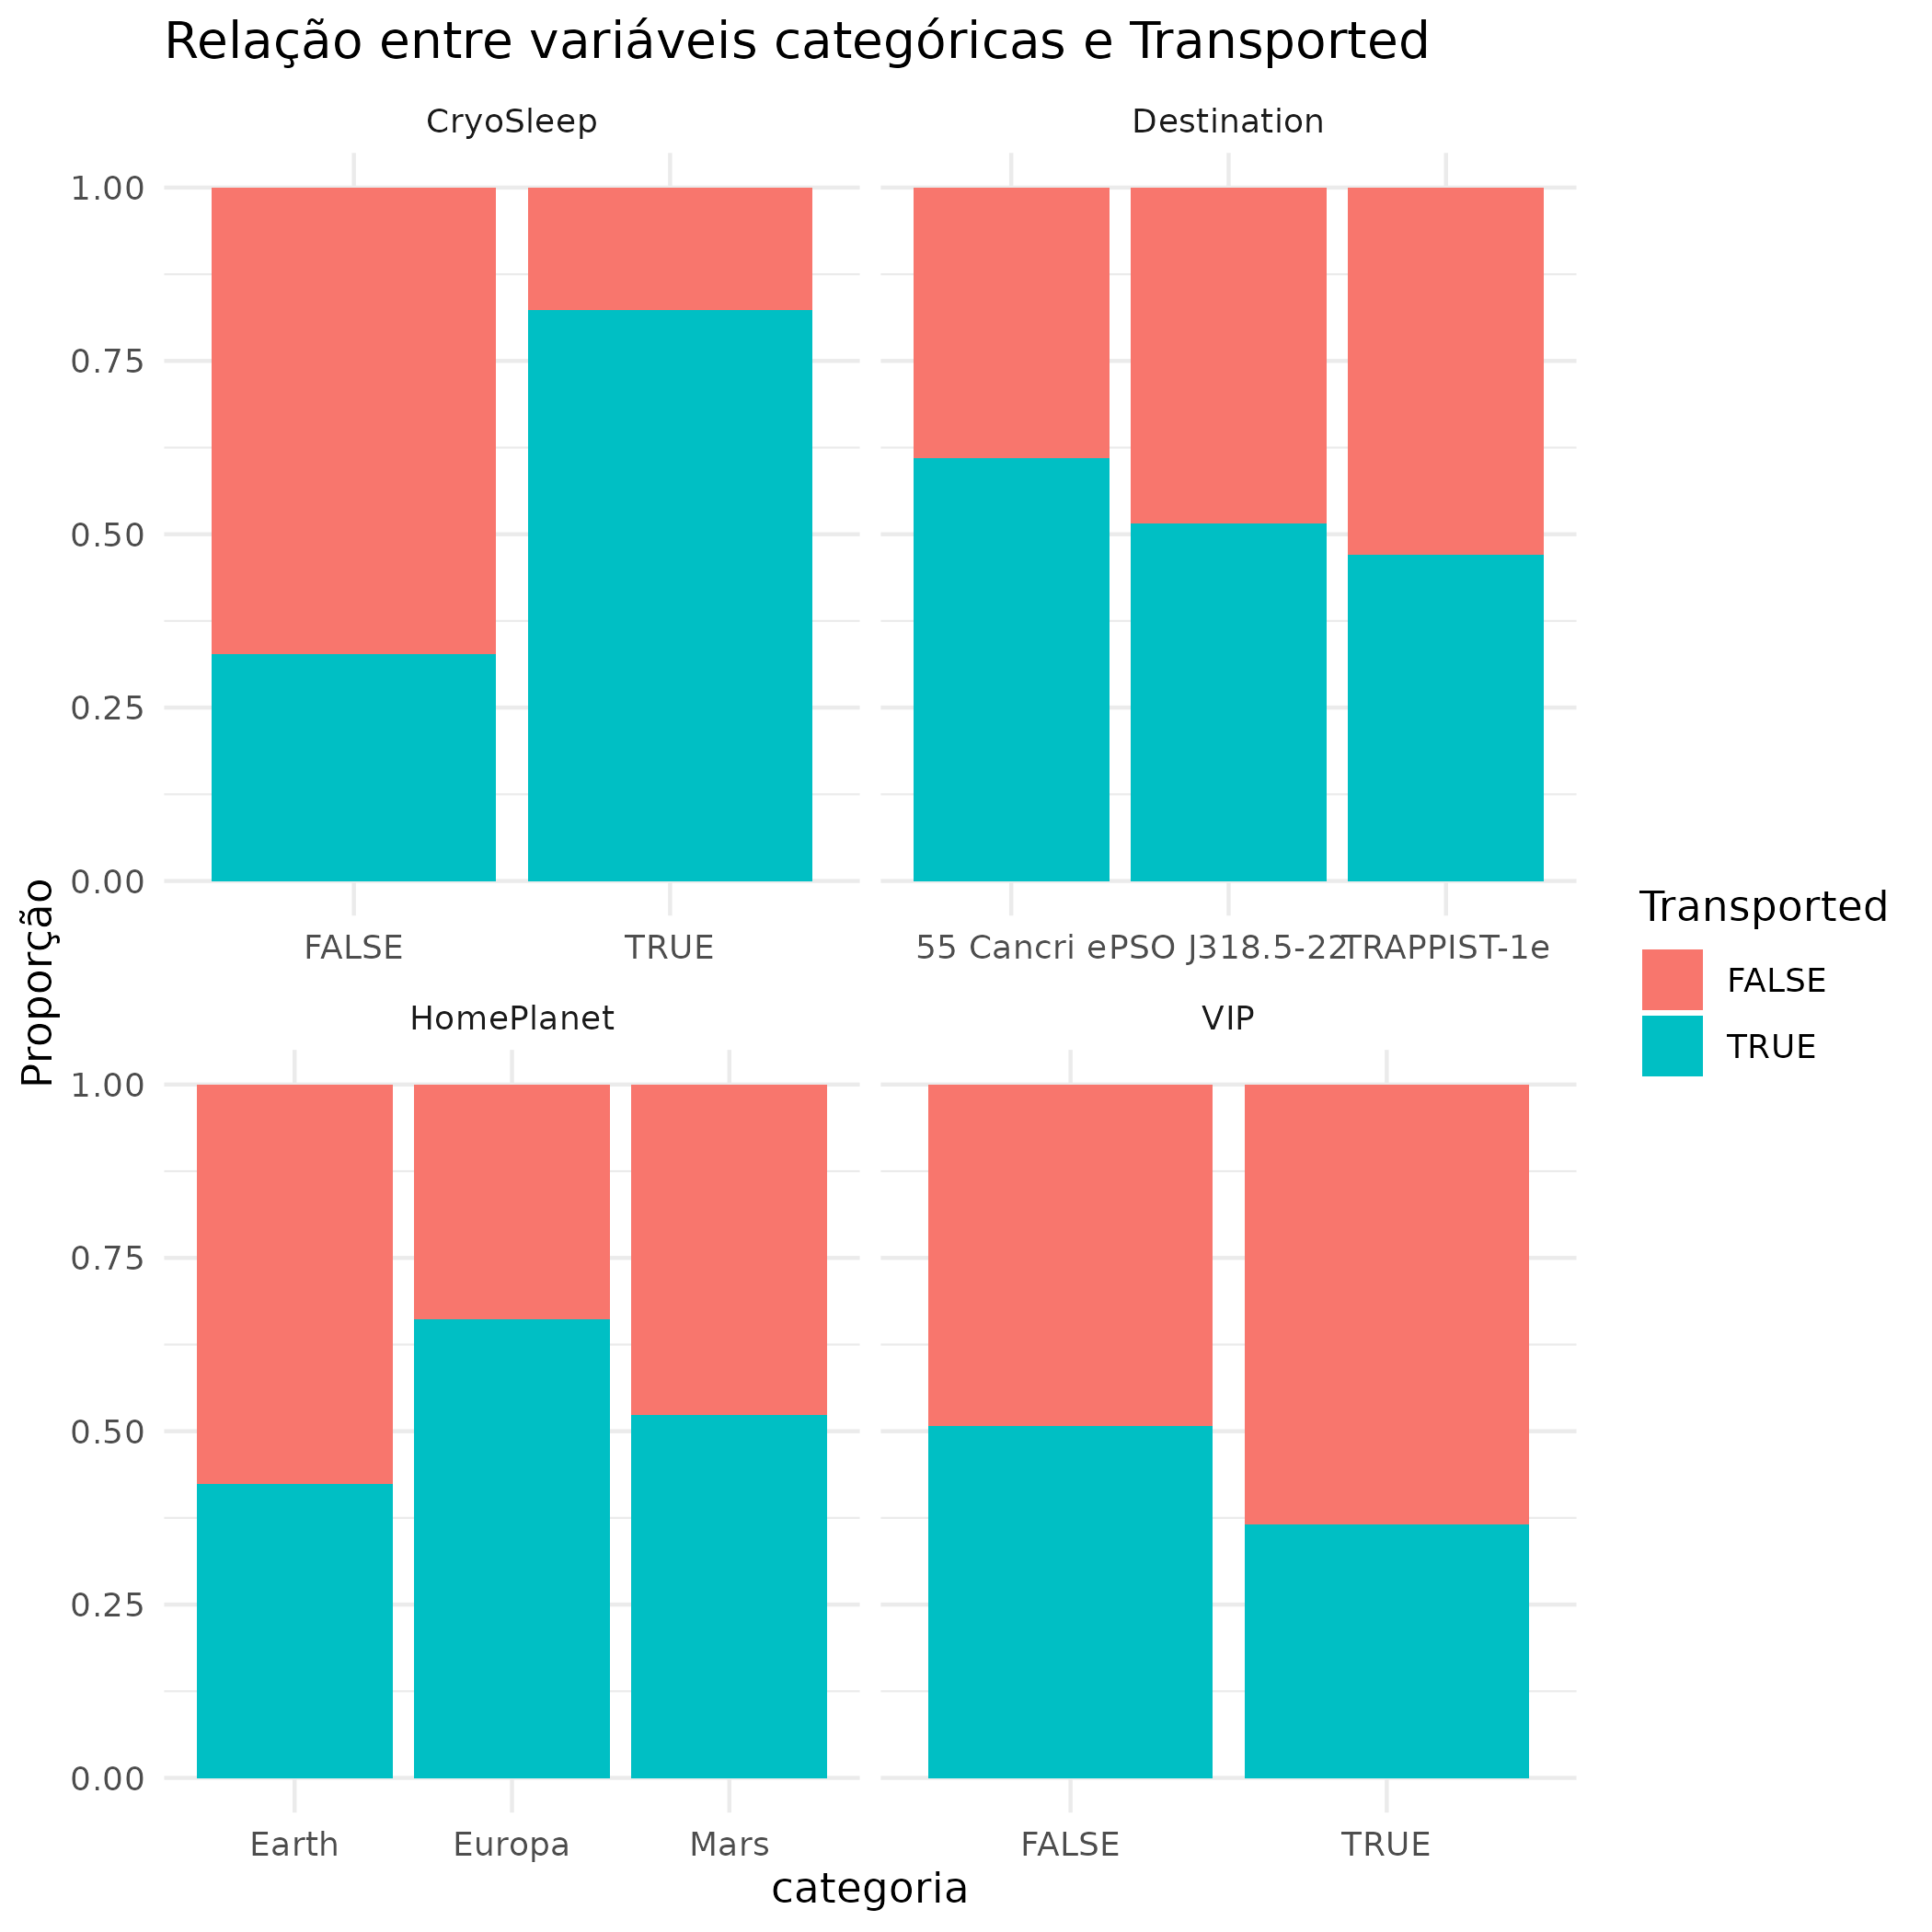
\includegraphics[width=.9\linewidth]{data/visualizations/barplots--Transported-vs-Categorical_Features.png}
\end{center}
\subsubsection{Análise Bivariada}
\label{sec:org3c56afd}
\paragraph{Exploração da coluna Cabin}
\label{sec:orgc2711fe}
\begin{verbatim}
cabin_data <- train_data %>%
  filter(!is.na(Cabin)) %>%
  mutate(deck = substr(Cabin, 1, 1)) %>%
  count(deck, Transported) %>%
  ggplot(aes(x = deck, y = n, fill = Transported)) +
  geom_col(position = "dodge") +
  theme_minimal()

print("Gerando análise bivariada para CabinDeck...")
ggsave(filename="data/visualizations/bivariate-analysis--cabin-deck.png",
       plot = cabin_data)
\end{verbatim}

\begin{center}
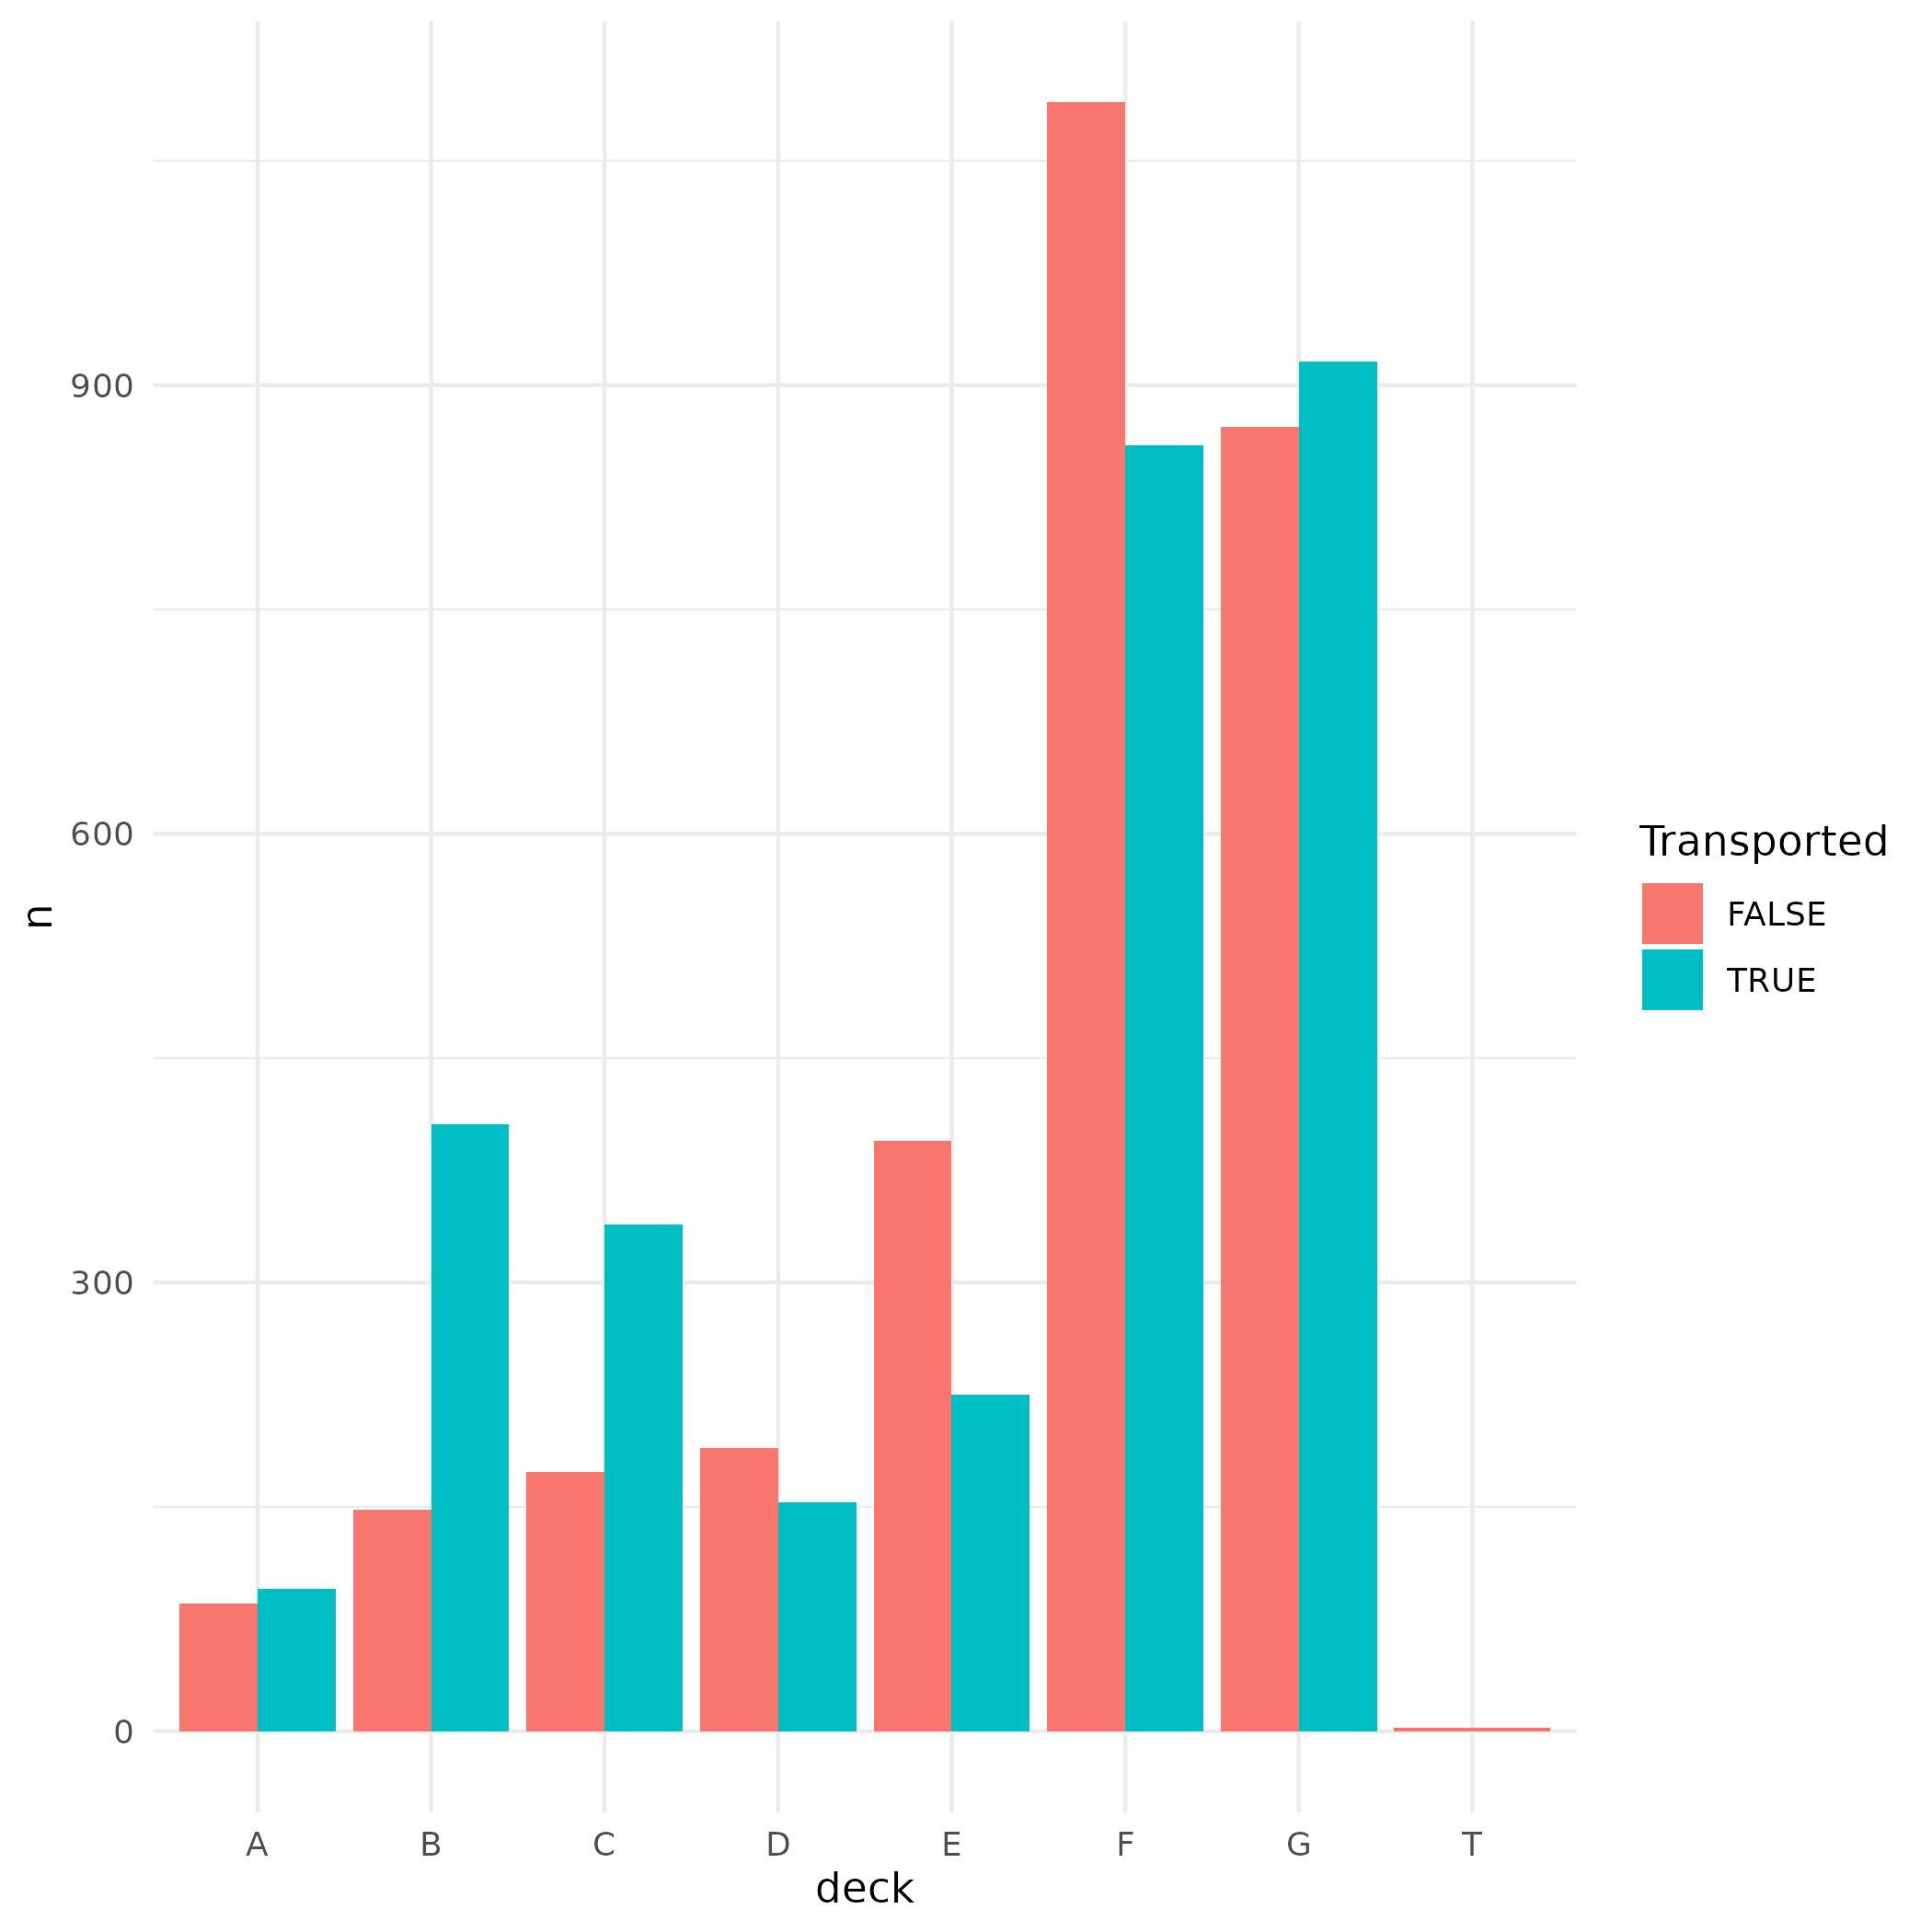
\includegraphics[width=.9\linewidth]{data/visualizations/bivariate-analysis--cabin-deck.png}
\end{center}
\section{Engenharia de \emph{Features}}
\label{sec:org6249f73}
\subsection{Adicionando \emph{Features}}
\label{sec:orgdd1f635}
\paragraph{Definição das \emph{Features} \texttt{Expenditure} e \texttt{NoExpenditure}}
\label{sec:orga915b4d}
A coluna \texttt{Expenditure} \textbf{agrupa} em si aditivamente os valores de custos dos tripulantes.
\begin{verbatim}
# Modificando os dados de treinamento para incluir =Expenditure=
train_data <- train_data %>%
  mutate(
    Expenditure = RoomService + FoodCourt + ShoppingMall + Spa + VRDeck,
  )

test_data <- test_data %>%
  mutate(
    Expenditure = RoomService + FoodCourt + ShoppingMall + Spa + VRDeck,
  )

# Incluindo =NoExpenditure=
train_data <- train_data %>%
  mutate(NoExpenditure = as.integer(Expenditure == 0))

test_data <- test_data %>%
  mutate(NoExpenditure = as.integer(Expenditure == 0))
\end{verbatim}

\begin{verbatim}
# Composição de gráficos para visualização da nova feature =Expenditure=
# 1. Histograma da despesa total
p_hist <- ggplot(train_data, aes(x = Expenditure)) +
  geom_histogram(fill = "steelblue", color = "white", bins = 40, alpha = 0.7) +
  scale_x_log10(labels = scales::comma) +  # escala log devido à assimetria
  labs(
    title = "Distribuição de Expenditure",
    x = "Gasto Total (escala log)",
    y = "Frequência"
  ) +
  theme_minimal()

# 2. Boxplot da despesa por status de transporte
p_box <- ggplot(train_data, aes(x = factor(Transported), y = Expenditure, fill = factor(Transported))) +
  geom_boxplot(alpha = 0.7, outlier.size = 0.8) +
  scale_y_log10(labels = scales::comma) +
  labs(
    title = "Expenditure por Transported",
    x = "Transportado",
    y = "Gasto Total (escala log)",
    fill = "Transportado"
  ) +
  theme_minimal() +
  theme(legend.position = "none")

# 3. Densidade (KDE) comparativa
p_density <- ggplot(train_data, aes(x = Expenditure, fill = factor(Transported))) +
  geom_density(alpha = 0.5) +
  scale_x_log10(labels = scales::comma) +
  labs(
    title = "Densidade de Expenditure por Classe",
    x = "Gasto Total (escala log)",
    y = "Densidade",
    fill = "Transportado"
  ) +
  theme_minimal()

# 4. Gráfico de barras para passageiros com gasto zero vs positivo
p_bar <- ggplot(train_data, aes(x = factor(NoExpenditure), fill = factor(Transported))) +
  geom_bar(position = "fill") +
  scale_y_continuous(labels = scales::percent) +
  scale_fill_manual(values = c("#E69F00", "#56B4E9")) +
  scale_x_discrete(labels = c("0" = "Com gastos", "1" = "Sem gastos")) +
  labs(title = "Proporção de Transportados por\nAusência de Gastos (NoExpenditure)",
       x = "",
       y = "Proporção") +
  theme_minimal()

# Combinar os gráficos em uma grade 2x2
composition <- (p_hist + p_box) / (p_density + p_bar) +
  plot_annotation(
    title = "Análise da Feature 'Expenditure'",
    theme = theme(plot.title = element_text(hjust = 0.5, size = 16, face = "bold"))
  )

# Salvar a composição
print("Gerando composição de gráficos da nova feature (Expenditure)...")
ggsave(filename = "data/visualizations/composition--Expenditure.png",
       plot = composition,
       width = 12, height = 10, dpi = 150)

# Gráfico 1: Contagem absoluta (barras lado a lado)
p_count <- ggplot(train_data, aes(x = factor(NoExpenditure), fill = factor(Transported))) +
  geom_bar(position = "dodge", alpha = 0.8) +
  scale_fill_manual(values = c("#E69F00", "#56B4E9"), 
                    name = "Transportado",
                    labels = c("Não", "Sim")) +
  scale_x_discrete(labels = c("0" = "Teve gastos", "1" = "Sem gastos")) +
  labs(title = "Contagem de passageiros por gasto zero",
       x = "No_spending (ausência de gastos)",
       y = "Contagem") +
  theme_minimal()

# Gráfico 2: Proporção dentro de cada categoria de No_spending (barras empilhadas 100%)
p_prop <- ggplot(train_data, aes(x = factor(NoExpenditure), fill = factor(Transported))) +
  geom_bar(position = "fill") +
  scale_y_continuous(labels = scales::percent) +
  scale_fill_manual(values = c("#E69F00", "#56B4E9"), 
                    name = "Transportado",
                    labels = c("Não", "Sim")) +
  scale_x_discrete(labels = c("0" = "Teve gastos", "1" = "Sem gastos")) +
  labs(title = "Proporção de transportados por ausência de gastos",
       x = "No_spending (ausência de gastos)",
       y = "Proporção") +
  theme_minimal()

# Combinar os dois gráficos lado a lado
composition_no_spending <- p_count + p_prop +
  plot_annotation(
    title = "Análise da Feature 'NoExpenditure'",
    theme = theme(plot.title = element_text(hjust = 0.5, size = 14, face = "bold"))
  )

# Salvar
print("Gerando composição de gráficos para feature 'NoExpenditure'...")
ggsave("data/visualizations/composition--NoExpenditure.png",
       plot = composition_no_spending, width = 12, height = 5, dpi = 150)
\end{verbatim}


\begin{center}
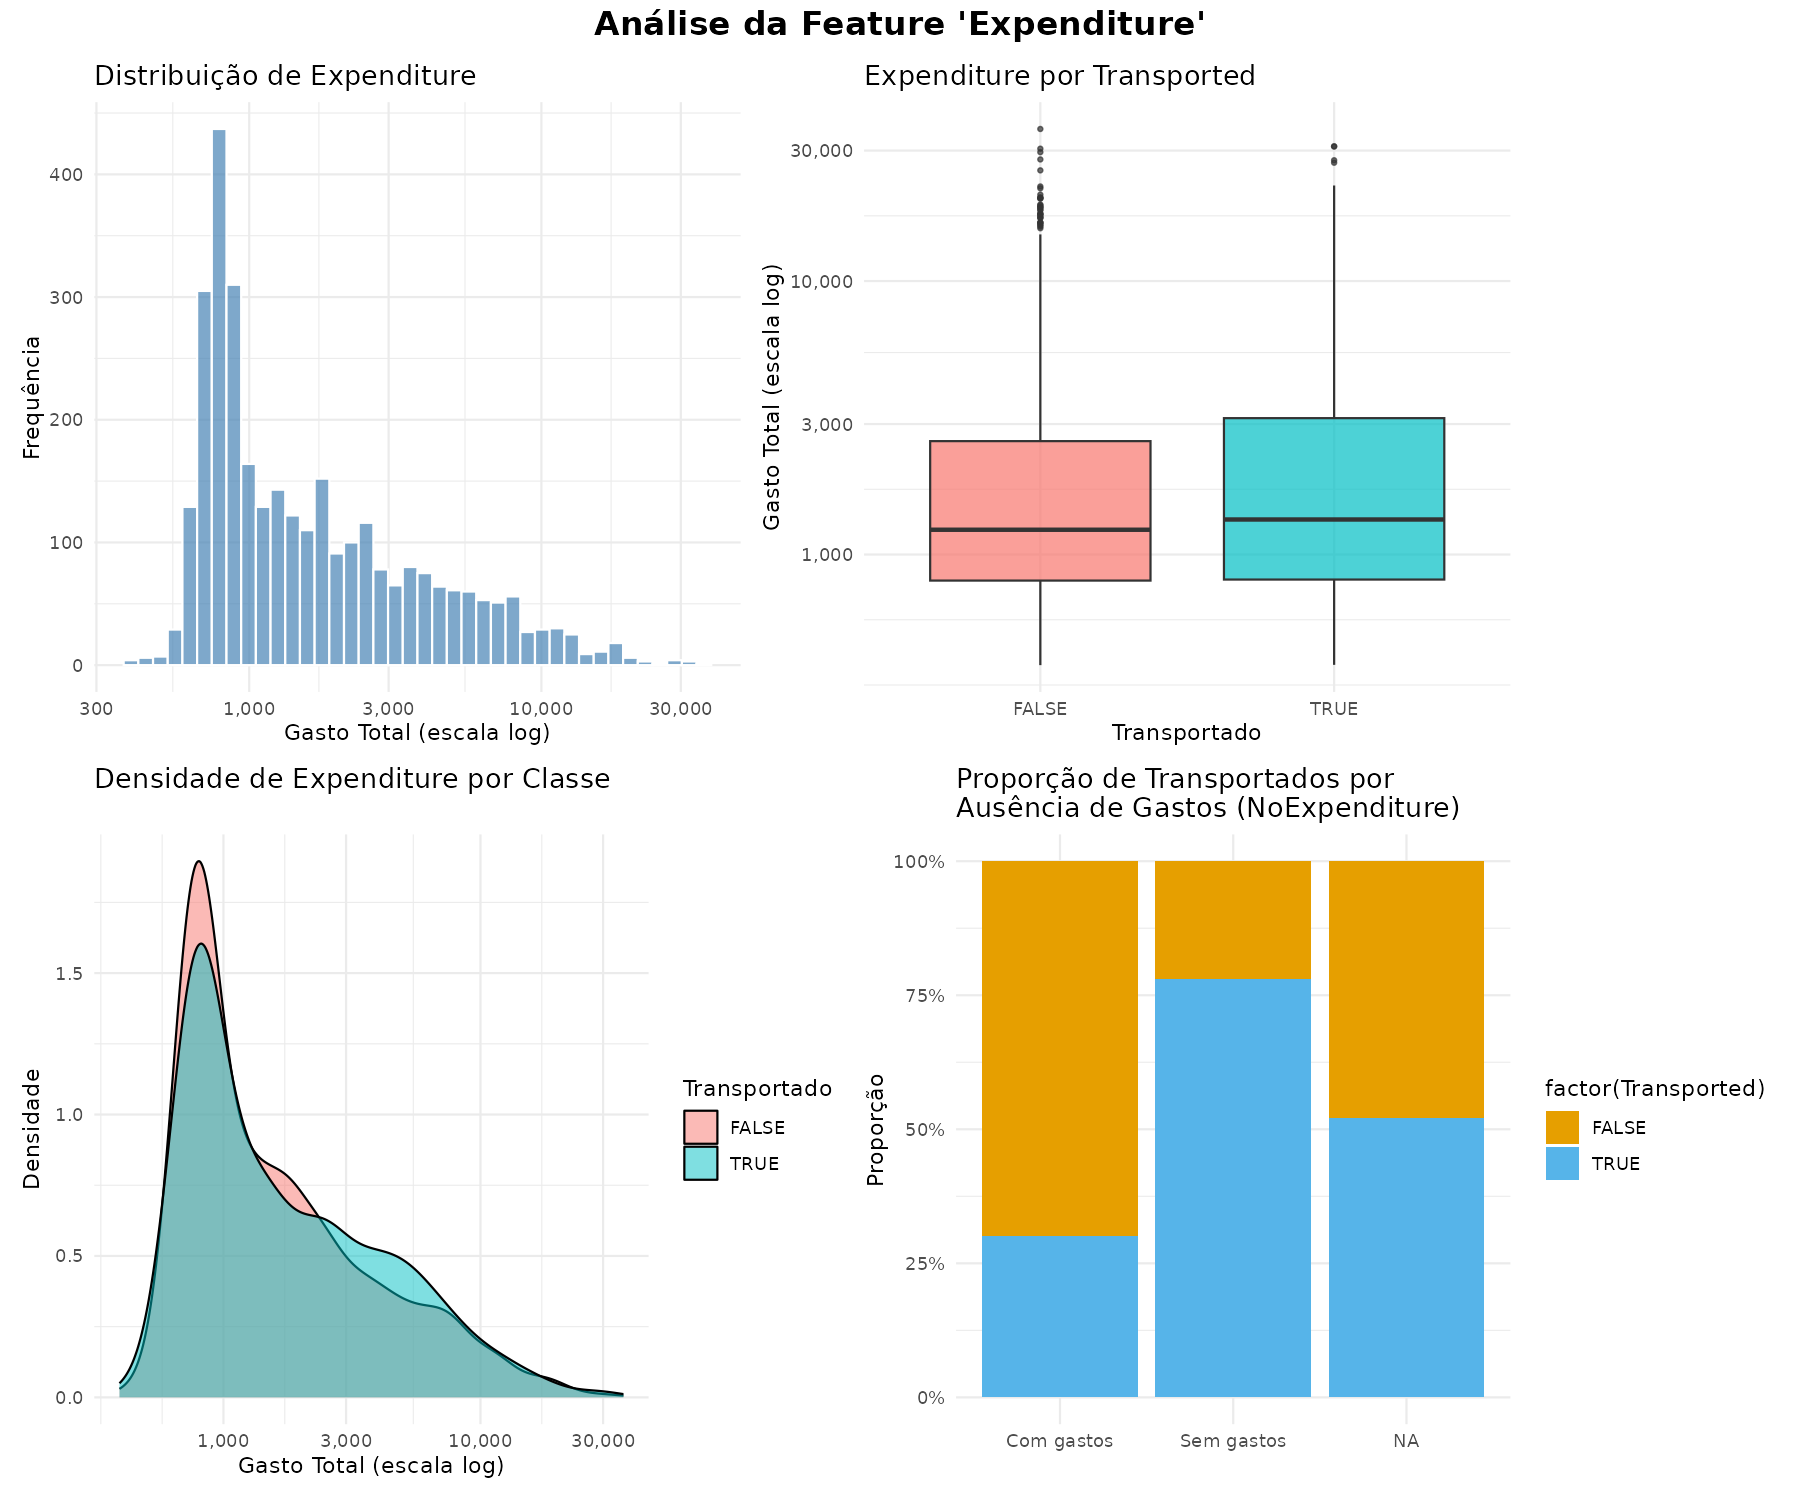
\includegraphics[width=.9\linewidth]{data/visualizations/composition--Expenditure.png}
\end{center}

\begin{center}
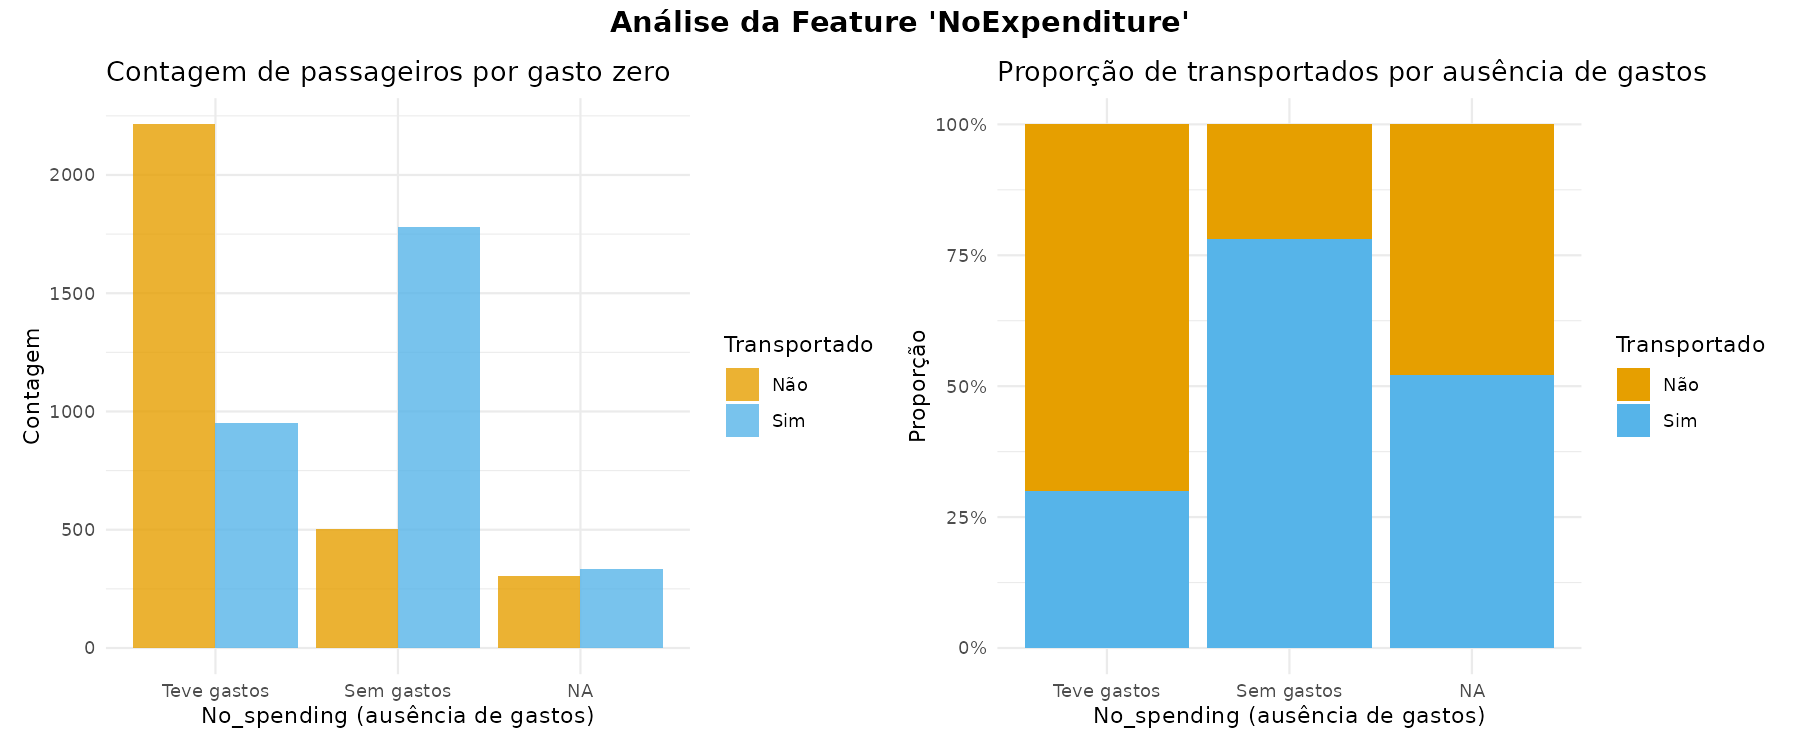
\includegraphics[width=.9\linewidth]{data/visualizations/composition--NoExpenditure.png}
\end{center}
\paragraph{Definição de \emph{Feature} \texttt{Age\_Group}}
\label{sec:org0ba228d}
Podemos discretizar a variação de idades do \emph{dataset} em grupos bem-definidos. Em seguida, veremos como essa discretização se reflete sobre nossa \emph{target}.

\begin{verbatim}
add_age_group <- function(df) {
  df %>%
    mutate(
      Age_Group = case_when(
        Age <= 12                     ~ "Age_0-12",
        Age > 12  & Age < 18          ~ "Age_13-17",
        Age >= 18 & Age <= 25         ~ "Age_18-25",
        Age > 25  & Age <= 30         ~ "Age_26-30",
        Age > 30  & Age <= 50         ~ "Age_31-50",
        Age > 50                      ~ "Age_51+",
        TRUE                          ~ NA_character_
      ),
      # Garantir que seja um fator com ordem correta
      Age_Group = factor(Age_Group, 
                         levels = c("Age_0-12", "Age_13-17", "Age_18-25",
                                    "Age_26-30", "Age_31-50", "Age_51+"))
    )
}

# Aplicar aos dados de treino e teste
train_data <- add_age_group(train_data)
test_data  <- add_age_group(test_data)
\end{verbatim}

\begin{verbatim}
# 1. Gráfico de barras (contagem absoluta) com hue = Transported
p1 <- ggplot(train_data, aes(x = Age_Group, fill = factor(Transported))) +
  geom_bar(position = "dodge", alpha = 0.8) +
  scale_fill_manual(values = c("#E69F00", "#56B4E9"), 
                    name = "Transportado",
                    labels = c("Não", "Sim")) +
  labs(
    title = "Distribuição dos Grupos Etários por Status de Transporte",
    x = "Grupo de Idade",
    y = "Contagem"
  ) +
  theme_minimal() +
  theme(axis.text.x = element_text(angle = 45, hjust = 1))

# 2. Gráfico de barras normalizado (proporção dentro de cada grupo)
p2 <- ggplot(train_data, aes(x = Age_Group, fill = factor(Transported))) +
  geom_bar(position = "fill", alpha = 0.8) +
  scale_y_continuous(labels = scales::percent) +
  scale_fill_manual(values = c("#E69F00", "#56B4E9"), 
                    name = "Transportado",
                    labels = c("Não", "Sim")) +
  labs(
    title = "Proporção de Transportados por Grupo Etário",
    x = "Grupo de Idade",
    y = "Proporção"
  ) +
  theme_minimal() +
  theme(axis.text.x = element_text(angle = 45, hjust = 1))

# 3. Boxplot da idade por grupo (para validar a categorização)
p3 <- ggplot(train_data, aes(x = Age_Group, y = Age, fill = factor(Transported))) +
  geom_boxplot(alpha = 0.7, outlier.size = 0.8) +
  scale_fill_manual(values = c("#E69F00", "#56B4E9"), 
                    name = "Transportado") +
  labs(
    title = "Distribuição da Idade por Grupo e Transporte",
    x = "Grupo de Idade",
    y = "Idade"
  ) +
  theme_minimal() +
  theme(axis.text.x = element_text(angle = 45, hjust = 1))

# 4. Gráfico de densidade da idade, destacando os grupos (facetado por Transported)
p4 <- ggplot(train_data, aes(x = Age, fill = Age_Group)) +
  geom_density(alpha = 0.6) +
  facet_wrap(~ Transported, labeller = labeller(Transported = c("TRUE" = "Transportado", "FALSE" = "Não transportado"))) +
  scale_fill_viridis_d() +
  labs(
    title = "Densidade da Idade por Grupo Etário e Status de Transporte",
    x = "Idade",
    y = "Densidade",
    fill = "Grupo de Idade"
  ) +
  theme_minimal()

# Combinar gráficos em uma grade 2x2
composition <- (p1 + p2) / (p3 + p4) +
  plot_annotation(
    title = "Análise da Feature 'Age_Group'",
    theme = theme(plot.title = element_text(hjust = 0.5, size = 16, face = "bold"))
  )

# Salvar a composição
print("Gerando composição de gráficos para feature Age_Group...")
ggsave("data/visualizations/composition--Age_Group.png", 
       plot = composition, width = 14, height = 10, dpi = 150)
\end{verbatim}

\begin{center}
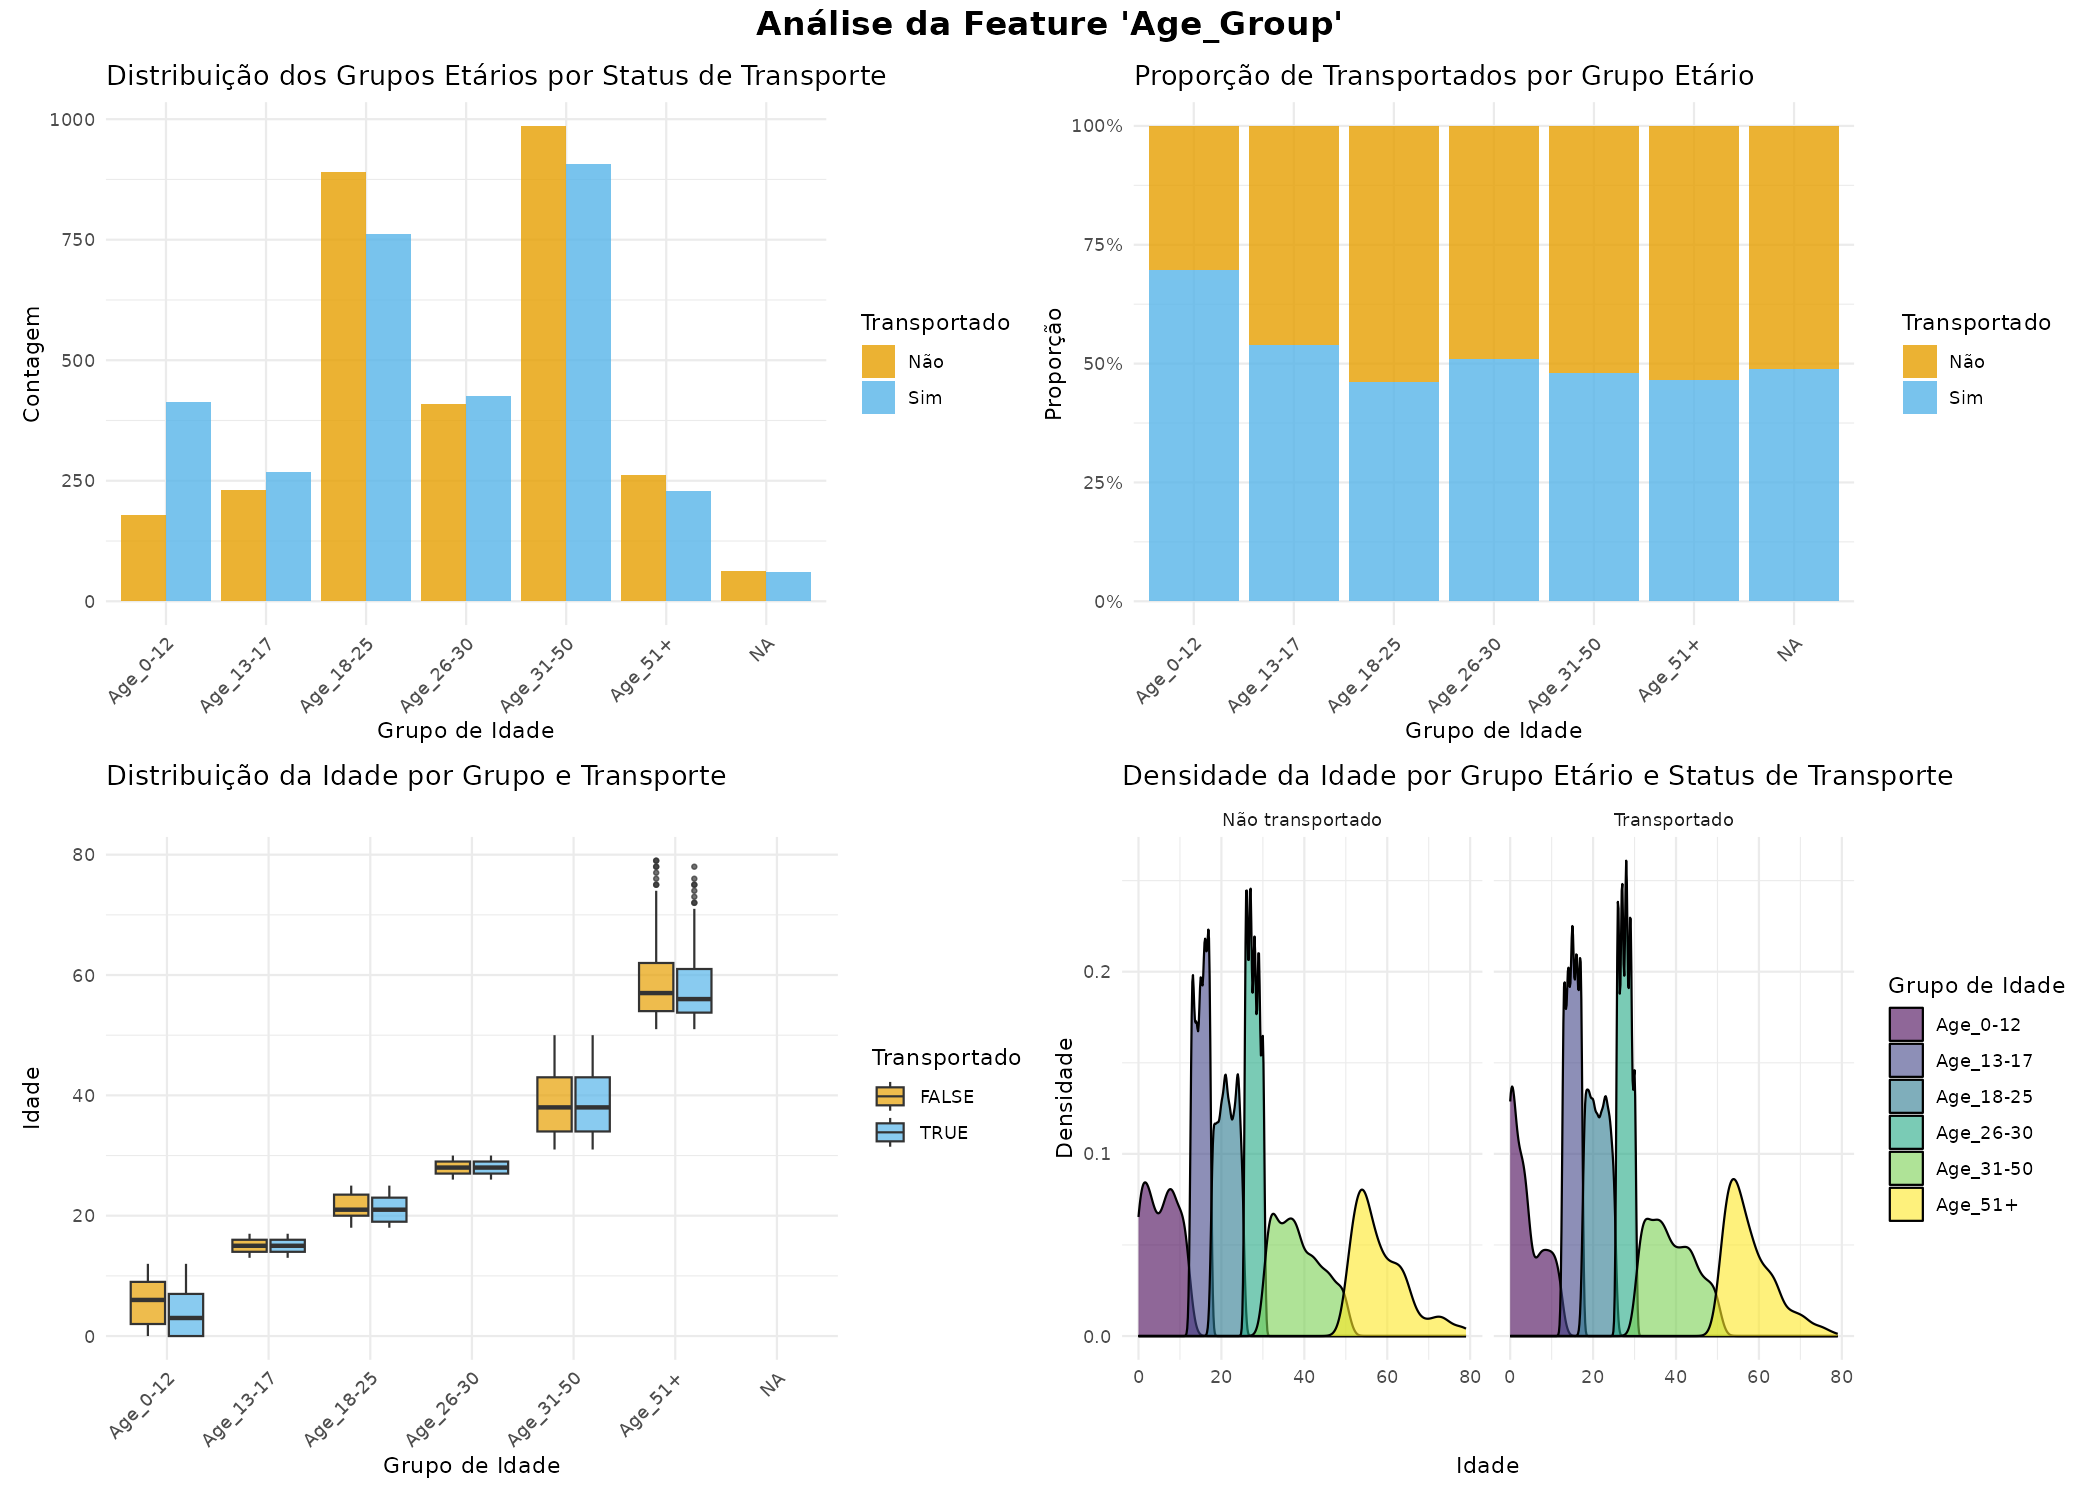
\includegraphics[width=.9\linewidth]{data/visualizations/composition--Age_Group.png}
\end{center}
\paragraph{Definição das \emph{Features} \texttt{Group} e \texttt{Group\_Size}}
\label{sec:org68fac4d}
A partir de \texttt{PassagerId}, podemos extrair a qual \emph{grupo} pertence um passageiro. Contando a quantidade de pessoas por grupo, podemos saber os tamanhos dos grupos.

\begin{verbatim}
# 1. Extrair 'Group' do PassengerId (antes do underscore)
train_data <- train_data %>%
  mutate(Group = as.integer(str_extract(PassengerId, "^[^_]+")))

test_data <- test_data %>%
  mutate(Group = as.integer(str_extract(PassengerId, "^[^_]+")))

# 2. Calcular 'Group_Size' usando contagem combinada de treino e teste
#    (mesma lógica do value_counts() em pandas)
combined_counts <- bind_rows(
  train_data %>% select(Group),
  test_data %>% select(Group)
) %>%
  count(Group, name = "Group_Size")

# Adicionar Group_Size aos dados de treino e teste via left_join
train_data <- train_data %>%
  left_join(combined_counts, by = "Group")

test_data <- test_data %>%
  left_join(combined_counts, by = "Group")
\end{verbatim}

\begin{verbatim}
# Gráfico 1: Histograma de Group (binwidth=1, hue=Transported)
p1 <- ggplot(train_data, aes(x = Group, fill = factor(Transported))) +
  geom_histogram(binwidth = 1, alpha = 0.7, position = "identity") +
  scale_fill_manual(values = c("#E69F00", "#56B4E9"), 
                    name = "Transportado",
                    labels = c("Não", "Sim")) +
  labs(title = "Group", x = "Grupo", y = "Contagem") +
  theme_minimal()

# Gráfico 2: Gráfico de barras (countplot) de Group_size, hue=Transported
p2 <- ggplot(train_data, aes(x = as.factor(Group_Size), fill = factor(Transported))) +
  geom_bar(position = "dodge", alpha = 0.8) +
  scale_fill_manual(values = c("#E69F00", "#56B4E9"), 
                    name = "Transportado",
                    labels = c("Não", "Sim")) +
  labs(title = "Group Size", x = "Tamanho do Grupo", y = "Contagem") +
  theme_minimal() +
  theme(axis.text.x = element_text(angle = 45, hjust = 1))

# Combinar os dois gráficos lado a lado (layout 1x2)
composition <- p1 + p2 +
  plot_annotation(
    title = "Distribuição das Features 'Group' e 'Group_Size'",
    theme = theme(plot.title = element_text(hjust = 0.5, size = 14, face = "bold"))
  )

# Salvar a composição (opcional)
if (!dir.exists("data/visualizations")) dir.create("data/visualizations", recursive = TRUE)
ggsave("data/visualizations/composition--Group_Group_Size.png", 
       plot = composition, width = 12, height = 5, dpi = 150)
\end{verbatim}

\begin{center}

\includegraphics[width=.9\linewidth]{data/visualizations/composition--Group_Group_size.png}
\end{center}
\paragraph{Definição da \emph{Feature} \texttt{Alone}}
\label{sec:org4aa13f0}
Se o \texttt{Group\_Size} ao qual pertence um passageiro é \texttt{1}, então o passageiro está viajando sozinho.


\begin{verbatim}
# Para o conjunto de treino
train_data <- train_data %>%
  mutate(Alone = as.integer(Group_Size == 1))

# Para o conjunto de teste
test_data <- test_data %>%
  mutate(Alone = as.integer(Group_Size == 1))
\end{verbatim}


\begin{verbatim}
# Gráfico 1: Barras lado a lado (contagem absoluta)
p1 <- ggplot(train_data, aes(x = factor(Alone), fill = factor(Transported))) +
  geom_bar(position = "dodge", alpha = 0.8) +
  scale_fill_manual(values = c("#E69F00", "#56B4E9"), 
                    name = "Transportado",
                    labels = c("Não", "Sim")) +
  scale_x_discrete(labels = c("0" = "Em grupo", "1" = "Sozinho")) +
  labs(title = "Contagem de passageiros viajando sozinhos ou em grupo",
       x = "Alone (viaja sozinho?)",
       y = "Contagem") +
  theme_minimal()

# Gráfico 2: Barras empilhadas (proporção dentro de cada categoria)
p2 <- ggplot(train_data, aes(x = factor(Alone), fill = factor(Transported))) +
  geom_bar(position = "fill") +
  scale_y_continuous(labels = scales::percent) +
  scale_fill_manual(values = c("#E69F00", "#56B4E9"), 
                    name = "Transportado",
                    labels = c("Não", "Sim")) +
  scale_x_discrete(labels = c("0" = "Em grupo", "1" = "Sozinho")) +
  labs(title = "Proporção de transportados por condição de viagem",
       x = "Alone (viaja sozinho?)",
       y = "Proporção") +
  theme_minimal()

# Combinar os dois gráficos lado a lado
composition_alone <- p1 + p2 +
  plot_annotation(
    title = "Análise da Feature 'Alone'",
    theme = theme(plot.title = element_text(hjust = 0.5, size = 14, face = "bold"))
  )

# Salvar a composição
print("Gerando composição de gráficos para feature 'Alone'...")
ggsave("data/visualizations/composition--Alone.png",
       plot = composition_alone, width = 12, height = 5, dpi = 150)
\end{verbatim}

\begin{center}
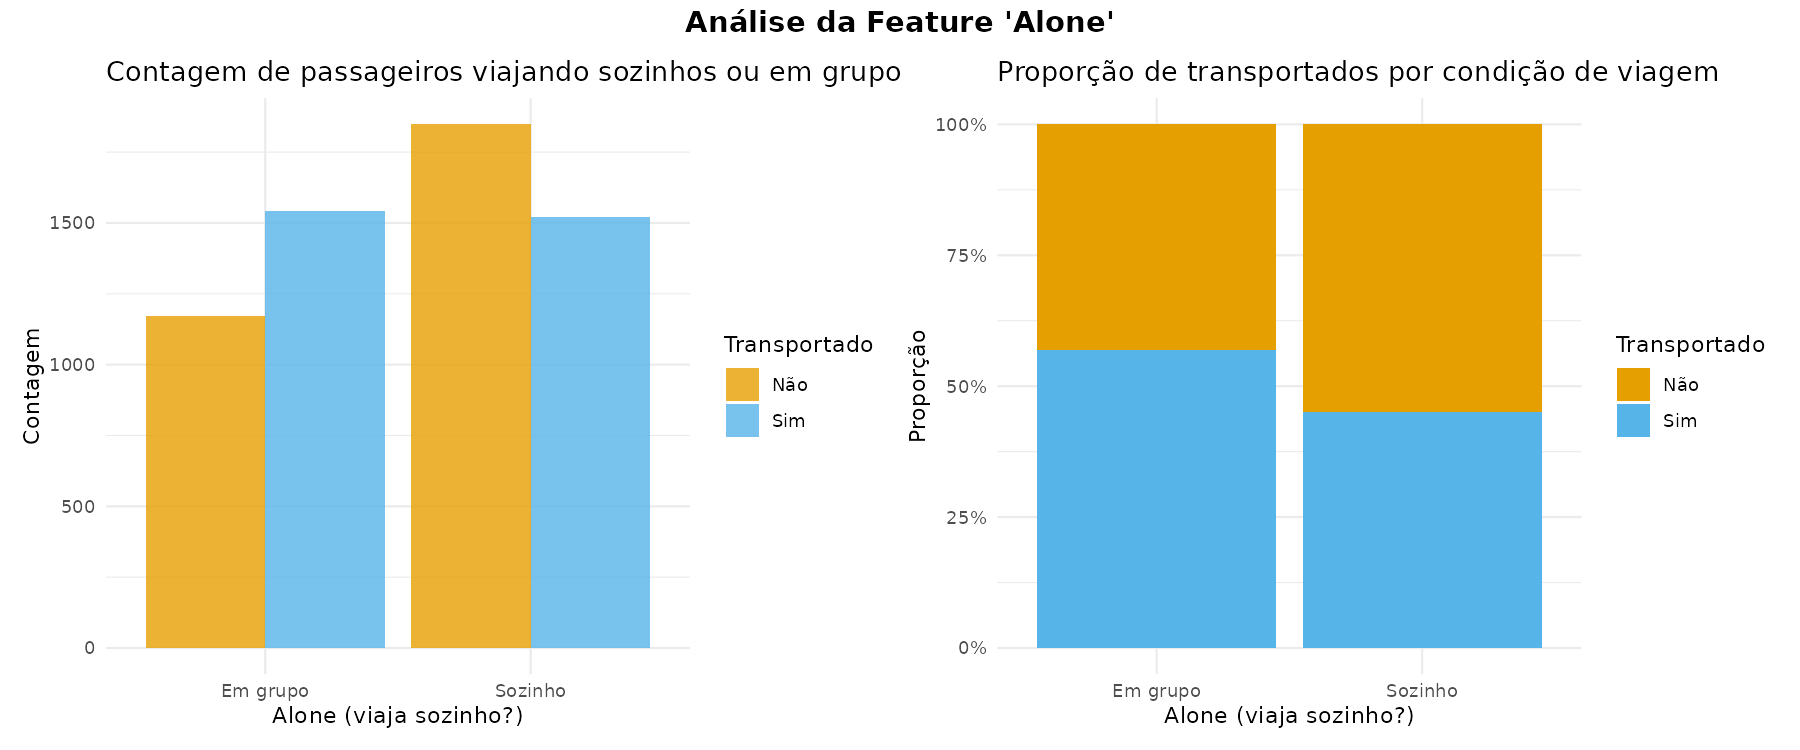
\includegraphics[width=.9\linewidth]{data/visualizations/composition--Alone.png}
\end{center}
\paragraph{Definição de \emph{Features} baseadas em \texttt{Cabin}: \texttt{Cabin\_Deck}, \texttt{Cabin\_Number}, \texttt{Cabin\_Side} e \texttt{Cabin\_RegionX}}
\label{sec:org2b85d9d}
Podemos analiar a \emph{feature} \texttt{Cabin} em três outras \emph{features} distintas.

\begin{verbatim}
# Substituir NA por um placeholder para permitir split
train_data <- train_data %>%
  mutate(Cabin = tidyr::replace_na(Cabin, "Z/9999/Z"))

test_data <- test_data %>%
  mutate(Cabin = tidyr::replace_na(Cabin, "Z/9999/Z"))

# Dividir a string Cabin em três componentes
train_data <- train_data %>%
  tidyr::separate(Cabin, into = c("Cabin_Deck", "Cabin_Number", "Cabin_Side"), 
                  sep = "/", remove = FALSE) %>%
  mutate(Cabin_Number = as.integer(Cabin_Number))

test_data <- test_data %>%
  tidyr::separate(Cabin, into = c("Cabin_Deck", "Cabin_Number", "Cabin_Side"), 
                  sep = "/", remove = FALSE) %>%
  mutate(Cabin_Number = as.integer(Cabin_Number))

# Recolocar NA nos placeholders
train_data <- train_data %>%
  mutate(Cabin_Deck   = if_else(Cabin_Deck == "Z",   NA_character_, Cabin_Deck),
         Cabin_Number = if_else(Cabin_Number == 9999, NA_integer_,  Cabin_Number),
         Cabin_Side   = if_else(Cabin_Side == "Z",   NA_character_, Cabin_Side))

test_data <- test_data %>%
  mutate(Cabin_Deck   = if_else(Cabin_Deck == "Z",   NA_character_, Cabin_Deck),
         Cabin_Number = if_else(Cabin_Number == 9999, NA_integer_,  Cabin_Number),
         Cabin_Side   = if_else(Cabin_Side == "Z",   NA_character_, Cabin_Side))

# Remover coluna Cabin original (não mais necessária)
train_data <- train_data %>% select(-Cabin)
test_data  <- test_data  %>% select(-Cabin)

# Criar regiões da cabine com base no número (Cabin_number)
# Bins: [0,300), [300,600), [600,900), [900,1200), [1200,1500), [1500,1800), [1800, Inf)
train_data <- train_data %>%
  mutate(
    Cabin_Region1 = as.integer(Cabin_Number < 300),
    Cabin_Region2 = as.integer(Cabin_Number >= 300 & Cabin_Number < 600),
    Cabin_Region3 = as.integer(Cabin_Number >= 600 & Cabin_Number < 900),
    Cabin_Region4 = as.integer(Cabin_Number >= 900 & Cabin_Number < 1200),
    Cabin_Region5 = as.integer(Cabin_Number >= 1200 & Cabin_Number < 1500),
    Cabin_Region6 = as.integer(Cabin_Number >= 1500 & Cabin_Number < 1800),
    Cabin_Region7 = as.integer(Cabin_Number >= 1800)
  )

test_data <- test_data %>%
  mutate(
    Cabin_Region1 = as.integer(Cabin_Number < 300),
    Cabin_Region2 = as.integer(Cabin_Number >= 300 & Cabin_Number < 600),
    Cabin_Region3 = as.integer(Cabin_Number >= 600 & Cabin_Number < 900),
    Cabin_Region4 = as.integer(Cabin_Number >= 900 & Cabin_Number < 1200),
    Cabin_Region5 = as.integer(Cabin_Number >= 1200 & Cabin_Number < 1500),
    Cabin_Region6 = as.integer(Cabin_Number >= 1500 & Cabin_Number < 1800),
    Cabin_Region7 = as.integer(Cabin_Number >= 1800)
  )

print("Features geradas a partir de 'Cabin': 'Cabin_Deck', 'Cabin_Number', 'Cabin_Side', 'Cabin_RegionX'")
\end{verbatim}

\begin{verbatim}
# 1. Gráfico de barras para Cabin_deck (ordem A-G, T)
deck_order <- c("A", "B", "C", "D", "E", "F", "G", "T")
p_deck <- ggplot(train_data, aes(x = factor(Cabin_Deck, levels = deck_order), 
                                  fill = factor(Transported))) +
  geom_bar(position = "dodge", alpha = 0.8) +
  scale_fill_manual(values = c("#E69F00", "#56B4E9"), 
                    name = "Transportado",
                    labels = c("Não", "Sim")) +
  labs(title = "Cabin Deck", x = "Deck", y = "Contagem") +
  theme_minimal() +
  theme(axis.text.x = element_text(angle = 0))

# 2. Histograma de Cabin_number com hue = Transported
p_number <- ggplot(train_data, aes(x = Cabin_Number, fill = factor(Transported))) +
  geom_histogram(binwidth = 20, alpha = 0.7, position = "identity") +
  scale_fill_manual(values = c("#E69F00", "#56B4E9"), 
                    name = "Transportado",
                    labels = c("Não", "Sim")) +
  geom_vline(xintercept = seq(300, 1800, by = 300), color = "black", linetype = "solid") +
  coord_cartesian(xlim = c(0, 2000)) +
  labs(title = "Cabin Number", x = "Número da Cabine", y = "Contagem") +
  theme_minimal()

# 3. Gráfico de barras para Cabin_side
p_side <- ggplot(train_data, aes(x = Cabin_Side, fill = factor(Transported))) +
  geom_bar(position = "dodge", alpha = 0.8) +
  scale_fill_manual(values = c("#E69F00", "#56B4E9"), 
                    name = "Transportado",
                    labels = c("Não", "Sim")) +
  labs(title = "Cabin Side", x = "Lado", y = "Contagem") +
  theme_minimal() +
  theme(axis.text.x = element_text(angle = 0))

# Empilhar os três primeiros gráficos verticalmente
top_plot <- (p_deck / p_number / p_side) +
  plot_annotation(title = "Análise das features derivadas de Cabin (Deck, Número, Lado)")

# 4. Gráfico para as regiões da cabine (criar variável combinada)
train_data <- train_data %>%
  mutate(Cabin_regions_plot = Cabin_Region1 * 1 +
                             Cabin_Region2 * 2 +
                             Cabin_Region3 * 3 +
                             Cabin_Region4 * 4 +
                             Cabin_Region5 * 5 +
                             Cabin_Region6 * 6 +
                             Cabin_Region7 * 7)

p_regions <- ggplot(train_data, aes(x = factor(Cabin_regions_plot), fill = factor(Transported))) +
  geom_bar(position = "dodge", alpha = 0.8) +
  scale_fill_manual(values = c("#E69F00", "#56B4E9"), 
                    name = "Transportado",
                    labels = c("Não", "Sim")) +
  labs(title = "Cabin regions (binas de número)", x = "Região", y = "Contagem") +
  theme_minimal() +
  theme(axis.text.x = element_text(angle = 0))

# Remover a coluna temporária (opcional, mas para não poluir o dataset)
train_data <- train_data %>% select(-Cabin_regions_plot)

# Salvar os gráficos individualmente ou em composição
print("Gerando composição de gráficos para features baseadas em 'Cabin'...")
ggsave("data/visualizations/cabin_deck_side_hist.png", 
       plot = top_plot, width = 8, height = 12, dpi = 150)
ggsave("data/visualizations/cabin_regions.png", 
       plot = p_regions, width = 8, height = 5, dpi = 150)
\end{verbatim}

\begin{center}
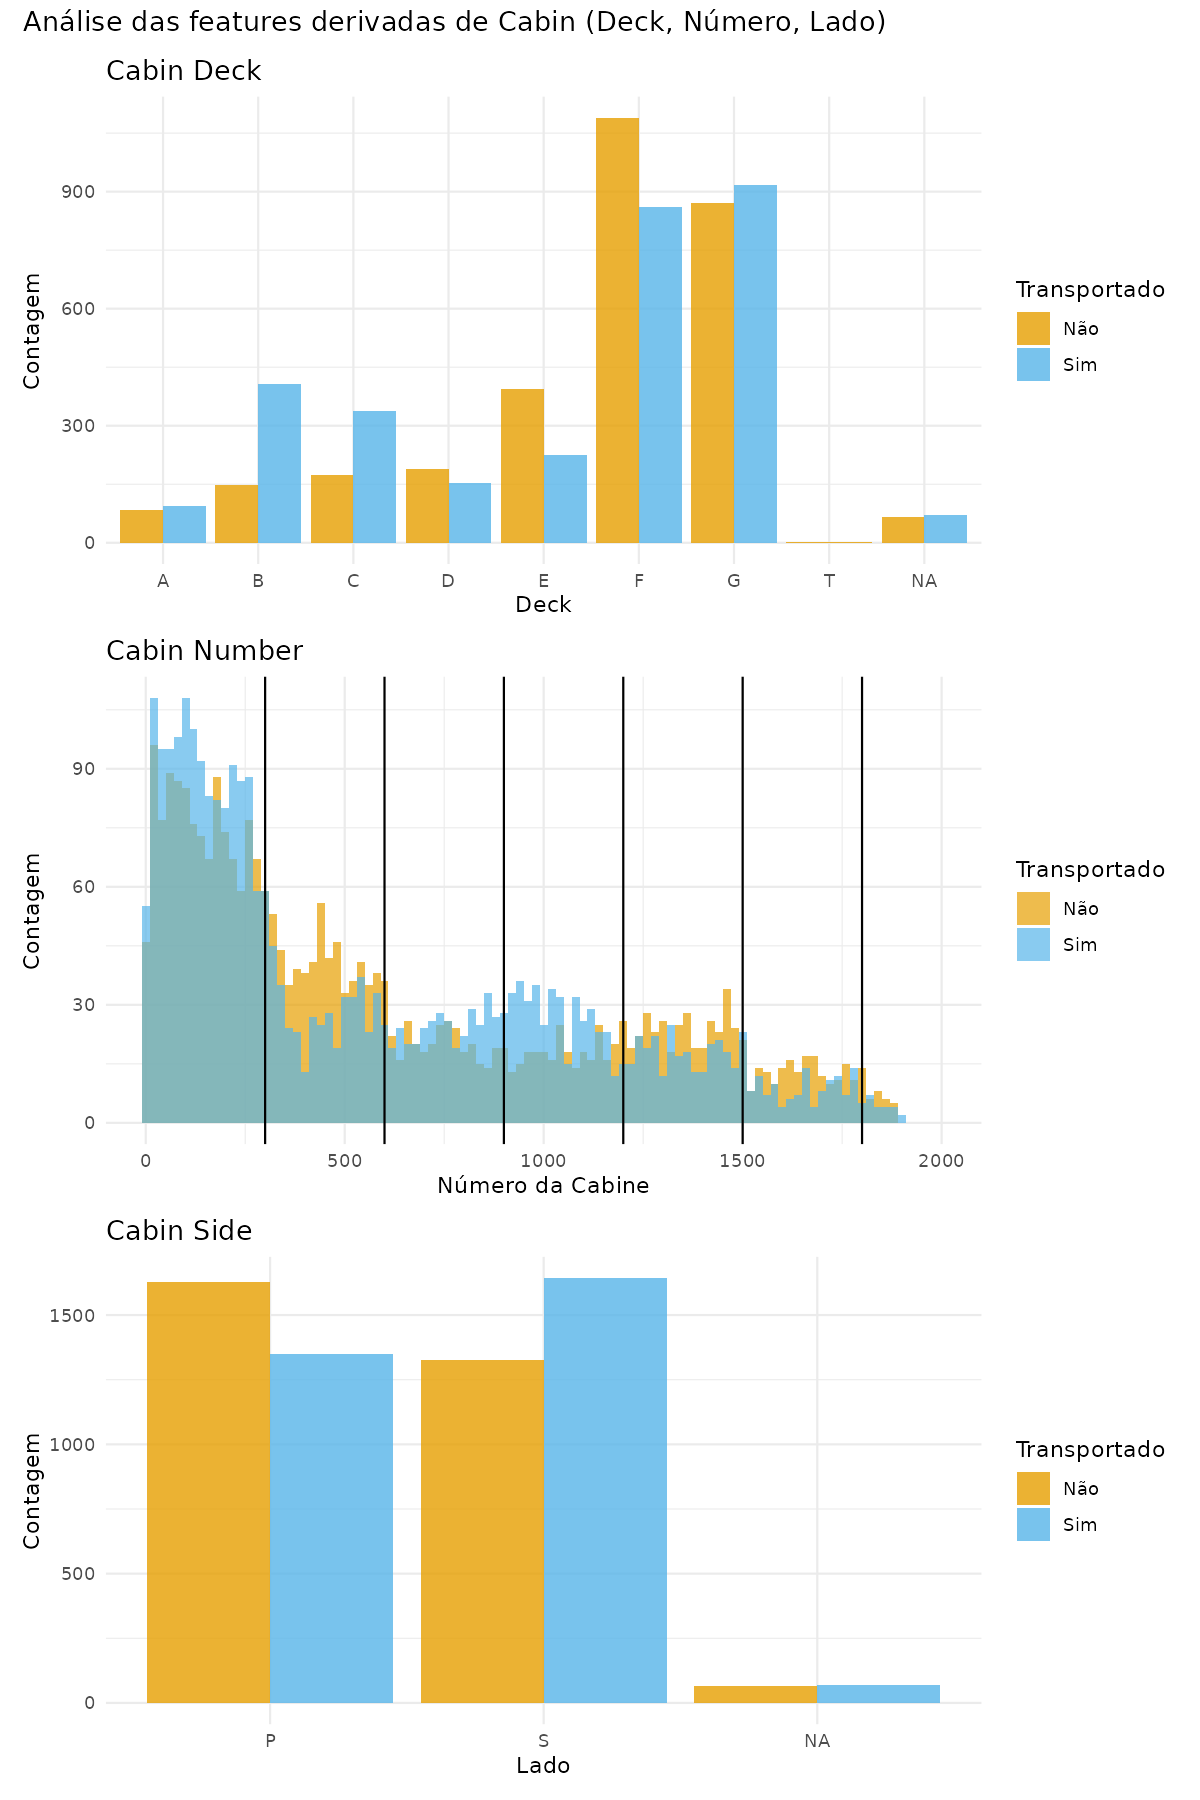
\includegraphics[width=.9\linewidth]{data/visualizations/cabin_deck_side_hist.png}
\end{center}
\begin{center}
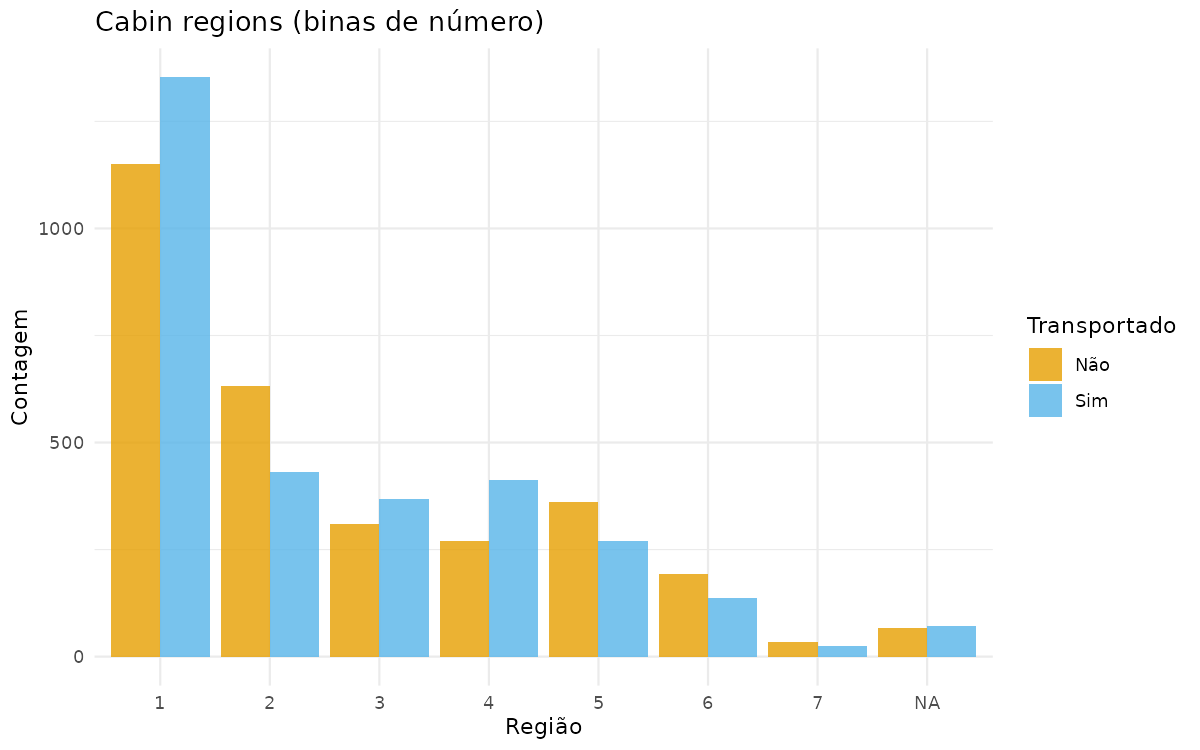
\includegraphics[width=.9\linewidth]{data/visualizations/cabin_regions.png}
\end{center}
\paragraph{Definição de \emph{Features} a partir de \texttt{Name}: \texttt{Family}, \texttt{FamilySize}}
\label{sec:orgf685398}
\begin{verbatim}
# 1. Substituir NA por placeholder "Unknown Unknown"
train_data <- train_data %>%
  mutate(Name = tidyr::replace_na(Name, "Unknown Unknown"))

test_data <- test_data %>%
  mutate(Name = tidyr::replace_na(Name, "Unknown Unknown"))

# 2. Extrair o sobrenome (última palavra do nome)
train_data <- train_data %>%
  mutate(Family = str_extract(Name, "\\S+$"))  # captura a última palavra

test_data <- test_data %>%
  mutate(Family = str_extract(Name, "\\S+$"))

# 3. Calcular Family_Size contando ocorrências do sobrenome em treino+teste
#    (mesma lógica do value_counts() no Python)
family_counts <- bind_rows(
  train_data %>% select(Family),
  test_data %>% select(Family)
) %>%
  count(Family, name = "Family_Size")

# Adicionar Family_Size aos dados
train_data <- train_data %>%
  left_join(family_counts, by = "Family")

test_data <- test_data %>%
  left_join(family_counts, by = "Family")

# 4. Recolocar NA nos placeholders (Unknown e valores > 100)
train_data <- train_data %>%
  mutate(
    Family = if_else(Family == "Unknown", NA_character_, Family),
    Family_Size = if_else(Family_Size > 100, NA_integer_, Family_Size)
  )

test_data <- test_data %>%
  mutate(
    Family = if_else(Family == "Unknown", NA_character_, Family),
    Family_Size = if_else(Family_Size > 100, NA_integer_, Family_Size)
  )

# 5. Remover a coluna original Name (não é mais necessária)
train_data <- train_data %>% select(-Name)
test_data  <- test_data  %>% select(-Name)
\end{verbatim}


\begin{verbatim}
# Converter Family_Size para fator (para countplot)
p_family <- ggplot(train_data, aes(x = factor(Family_Size), fill = factor(Transported))) +
  geom_bar(position = "dodge", alpha = 0.8) +
  scale_fill_manual(values = c("#E69F00", "#56B4E9"), 
                    name = "Transportado",
                    labels = c("Não", "Sim")) +
  labs(title = "Family size", x = "Tamanho da família", y = "Contagem") +
  theme_minimal() +
  theme(axis.text.x = element_text(angle = 45, hjust = 1))

# Salvar o gráfico (opcional)
print("Gerando barplot para 'Family_Size'...")
ggsave("data/visualizations/family_size_distribution.png", 
       plot = p_family, width = 8, height = 5, dpi = 150)
\end{verbatim}

\begin{center}
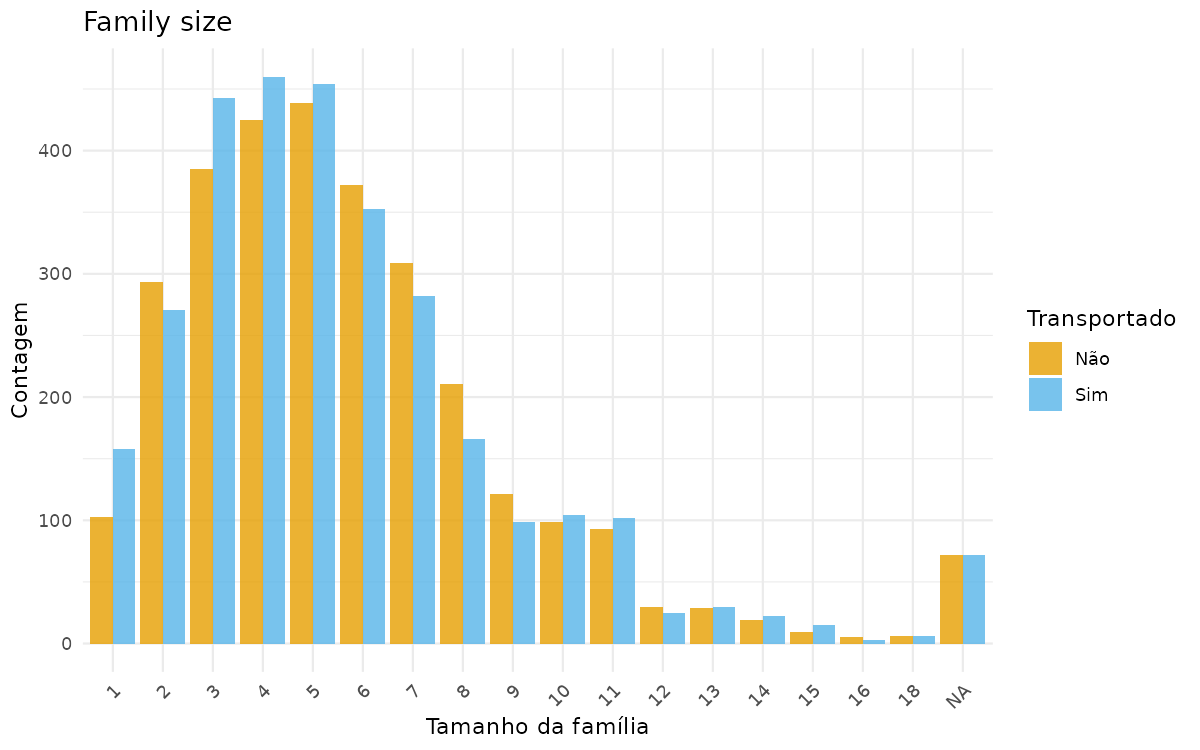
\includegraphics[width=.9\linewidth]{data/visualizations/family_size_distribution.png}
\end{center}
\subsection{Realizando Testes}
\label{sec:orgdc778ea}
\subsubsection{\texttt{ttest}}
\label{sec:orgfb1f739}
\begin{verbatim}
perform_ttest <- function(train, feature_list, target) {
  # Cria um data.frame vazio para armazenar os resultados
  results <- data.frame(
    Feature = character(),
    t_stat  = numeric(),
    p_val   = numeric(),
    stringsAsFactors = FALSE
  )

  for (feat in feature_list) {
    # Constrói a fórmula: feature ~ target
    formula <- as.formula(paste(feat, "~", target))
    # Aplica o teste t com exclusão de NAs
    test <- t.test(formula, data = train, na.action = na.omit)

    # Adiciona os resultados
    results <- rbind(results, data.frame(
      Feature = feat,
      t_stat  = test$statistic,
      p_val   = test$p.value
    ))
  }

  # Exibe a tabela formatada (semelhante ao PrettyTable)
  print(knitr::kable(results, digits = 4, caption = "Resultados do teste t"))
}

cont_cols <- c("Age", "Expenditure", "RoomService", "FoodCourt", "ShoppingMall", "Spa", "VRDeck")

# Executar a função nos dados de treino
print("Aplicando ttest às features numéricas...");
perform_ttest(train_data, cont_cols, "Transported")
\end{verbatim}
\subsubsection{\texttt{ANOVA}}
\label{sec:org8d8d5b0}
\begin{verbatim}
perform_anova <- function(train, feature_list, target) {
  # Cria um data.frame vazio para armazenar os resultados
  results <- data.frame(
    Feature = character(),
    F_statistic = numeric(),
    p_value = numeric(),
    stringsAsFactors = FALSE
  )

  for (feat in feature_list) {
    # Constrói a fórmula: feature ~ target
    formula <- as.formula(paste(feat, "~", target))
    # Ajusta o modelo linear e extrai a ANOVA (type I)
    model <- lm(formula, data = train, na.action = na.omit)
    anova_summary <- summary(aov(model))
    f_stat <- anova_summary[[1]]$`F value`[1]
    p_val  <- anova_summary[[1]]$`Pr(>F)`[1]

    # Adiciona os resultados
    results <- rbind(results, data.frame(
      Feature = feat,
      F_statistic = f_stat,
      p_value = p_val
    ))
  }

  # Exibe a tabela formatada
  print(knitr::kable(results, digits = 4, caption = "Resultados da ANOVA one-way"))
}

cont_cols <- c("Age", "Expenditure", "RoomService", "FoodCourt", 
               "ShoppingMall", "Spa", "VRDeck")

# Executar a função nos dados de treino
print("Aplicando ANOVA às features numéricas...")
perform_anova(train_data, cont_cols, "Transported")
\end{verbatim}
\subsection{Imputação e Transformação de Dados}
\label{sec:org78e83b9}
\subsubsection{Imputando dados a partir das conclusões anteriores}
\label{sec:org234992e}
\begin{verbatim}
exp_features <- c(
  "RoomService",
  "FoodCourt",
  "ShoppingMall",
  "Spa",
  "VRDeck"
)

# Criar feature agregada de gastos de novo
train_data <- train_data %>%
  mutate(
    Expenditure = rowSums(
      across(all_of(exp_features)),
      na.rm = TRUE
    )
  )

test_data <- test_data %>%
  mutate(
    Expenditure = rowSums(
      across(all_of(exp_features)),
      na.rm = TRUE
    )
  )

# Imputar CryoSleep SOMENTE onde NA
train_data <- train_data %>%
  mutate(
    CryoSleep = case_when(
      !is.na(CryoSleep) ~ CryoSleep,
      Expenditure == 0 ~ TRUE,
      Expenditure > 0  ~ FALSE,
      TRUE ~ NA
    )
  )

test_data <- test_data %>%
  mutate(
    CryoSleep = case_when(
      !is.na(CryoSleep) ~ CryoSleep,
      Expenditure == 0 ~ TRUE,
      Expenditure > 0  ~ FALSE,
      TRUE ~ NA
    )
  )

# Ajustar gastos de passageiros em CryoSleep
train_data <- train_data %>%
  mutate(
    across(
      all_of(exp_features),
      ~ ifelse(CryoSleep == TRUE, 0, .x)
    )
  )

test_data <- test_data %>%
  mutate(
    across(
      all_of(exp_features),
      ~ ifelse(CryoSleep == TRUE, 0, .x)
    )
  )

# VIP: imputação conservadora
train_data <- train_data %>%
  mutate(
    VIP = case_when(
      !is.na(VIP) ~ VIP,
      Expenditure > quantile(Expenditure, 0.90, na.rm = TRUE) ~ TRUE,
      TRUE ~ FALSE
    )
  )

test_data <- test_data %>%
  mutate(
    VIP = case_when(
      !is.na(VIP) ~ VIP,
      Expenditure > quantile(Expenditure, 0.90, na.rm = TRUE) ~ TRUE,
      TRUE ~ FALSE
    )
  )

# Guardar PassengerId
pid_train <- train_data$PassengerId
pid_test  <- test_data$PassengerId

train_data <- train_data %>%
  select(-PassengerId)

test_data <- test_data %>%
  select(-PassengerId)

# Função robusta de imputação KNN
impute_knn <- function(df, k = 5) {
  numeric_cols <- df %>%
    select(where(is.numeric)) %>%
    names()

  data_num <- df[, numeric_cols, drop = FALSE]

  # Preencher temporariamente NAs com mediana
  temp_data <- data_num %>%
    mutate(
      across(
        everything(),
        ~ ifelse(
          is.na(.x),
          median(.x, na.rm = TRUE),
          .x
        )
      )
    )

  # Imputar coluna por coluna
  for (col in numeric_cols) {
    missing_idx <- which(is.na(data_num[[col]]))

    if (length(missing_idx) == 0)
      next

    predictor_cols <- setdiff(numeric_cols, col)

    train_matrix <- temp_data[
      !is.na(data_num[[col]]),
      predictor_cols,
      drop = FALSE
    ]

    query_matrix <- temp_data[
      missing_idx,
      predictor_cols,
      drop = FALSE
    ]

    nn <- nn2(
      data = train_matrix,
      query = query_matrix,
      k = k
    )

    target_values <- data_num[[col]]

    imputed <- apply(
      nn$nn.idx,
      1,
      function(idx) {
        mean(
          target_values[!is.na(target_values)][idx],
          na.rm = TRUE
        )
      }
    )

    data_num[[col]][missing_idx] <- imputed
  }

  df[, numeric_cols] <- data_num

  return(df)
}


# Imputação conjunta (melhor distribuição)
train_rows <- nrow(train_data)

combined_data <- bind_rows(
  train_data,
  test_data
)

combined_data <- impute_knn(
  combined_data,
  k = 5
)

train_data <- combined_data[1:train_rows, ]
test_data  <- combined_data[(train_rows + 1):nrow(combined_data), ]

# Restaurar PassengerId
train_data$PassengerId <- pid_train
test_data$PassengerId  <- pid_test

print("Imputação de valores ausentes com KNN terminada...")
\end{verbatim}
\subsubsection{Transformações Numéricas e Seleção por Validação Cruzada}
\label{sec:orgcc38087}
\begin{verbatim}
# Features numéricas originais
orig_numerics <- c(
  "Age",
  "RoomService",
  "FoodCourt",
  "ShoppingMall",
  "Spa",
  "VRDeck",
  "Group",
  "Cabin_Number",
  "Expenditure"
)

orig_numerics <- intersect(
  orig_numerics,
  names(train_data)
)

# Função de avaliação
cv_accuracy <- function(df, feature, target = "Transported", k = 5) {
  formula <- as.formula(
    paste(target, "~", feature)
  )

  folds <- createFolds(
    df[[target]],
    k = k,
    returnTrain = FALSE
  )

  scores <- c()

  for (idx in folds) {
    train_fold <- df[-idx, ]
    val_fold   <- df[idx, ]

    model <- glm(
      formula,
      data = train_fold,
      family = binomial()
    )

    probs <- predict(
      model,
      newdata = val_fold,
      type = "response"
    )

    preds <- probs > 0.5

    acc <- mean(
      preds == val_fold[[target]]
    )

    scores <- c(scores, acc)
  }

  mean(scores)
}

# Aplicar transformações
best_features <- list()

for (orig in orig_numerics) {
  cat("\nProcessando:", orig, "\n")
  # Validar coluna
  if (!is.numeric(train_data[[orig]])) {
    next
  }

  # Features derivadas
  train_temp <- train_data
  test_temp  <- test_data

  # Original
  train_temp[[paste0(orig, "_orig")]] <- train_temp[[orig]]
  test_temp[[paste0(orig, "_orig")]]  <- test_temp[[orig]]

  # Log
  if (all(train_temp[[orig]] >= 0, na.rm = TRUE)) {

    train_temp[[paste0(orig, "_log")]] <-
      log1p(train_temp[[orig]])

    test_temp[[paste0(orig, "_log")]] <-
      log1p(test_temp[[orig]])
  }

  # Sqrt
  if (all(train_temp[[orig]] >= 0, na.rm = TRUE)) {

    train_temp[[paste0(orig, "_sqrt")]] <-
      sqrt(train_temp[[orig]])

    test_temp[[paste0(orig, "_sqrt")]] <-
      sqrt(test_temp[[orig]])
  }

  # Square
  train_temp[[paste0(orig, "_sq")]] <-
    train_temp[[orig]]^2

  test_temp[[paste0(orig, "_sq")]] <-
    test_temp[[orig]]^2

  # Yeo-Johnson
  yj_model <- yeojohnson(train_temp[[orig]])

  train_temp[[paste0(orig, "_yj")]] <-
    predict(yj_model)

  test_temp[[paste0(orig, "_yj")]] <-
    predict(
      yj_model,
      newdata = test_temp[[orig]]
    )

  # Avaliar features
  candidates <- names(train_temp) %>%
    grep(
      paste0("^", orig, "_"),
      .,
      value = TRUE
    )

  scores <- sapply(
    candidates,
    function(f) {
      cv_accuracy(
        train_temp[, c(f, "Transported")],
        f
      )
    }
  )

  best_feature <- names(scores)[which.max(scores)]
  best_score   <- max(scores)

  cat(
    "Melhor:",
    best_feature,
    "| acc =",
    round(best_score, 5),
    "\n"
  )

  best_features[[orig]] <- best_feature

  # Manter apenas a melhor
  train_data[[best_feature]] <-
    train_temp[[best_feature]]

  test_data[[best_feature]] <-
    test_temp[[best_feature]]

  # Remover original
  train_data[[orig]] <- NULL
  test_data[[orig]]  <- NULL
}

# Limpeza final
# Remover colunas constantes
constant_cols <- names(train_data)[
  sapply(train_data, function(x)
    length(unique(x)) <= 1)
]

train_data <- train_data %>%
  select(-all_of(constant_cols))

test_data <- test_data %>%
  select(-any_of(constant_cols))

# Converter lógicos
train_data <- train_data %>%
  mutate(
    across(
      where(is.logical),
      as.integer
    )
  )

test_data <- test_data %>%
  mutate(
    across(
      where(is.logical),
      as.integer
    )
  )

cat("\nTransformações finalizadas.\n")
\end{verbatim}
\section{Exportando os Dados Processados}
\label{sec:org9f00e8d}
\subsection{Visualizando o que foi feito}
\label{sec:org0cda848}
\begin{verbatim}
cat("\n==============================\n")
cat("COLUNAS FINAIS - TREINO\n")
cat("==============================\n\n")

print(names(train_data))

cat("\nTotal de colunas treino:",
    ncol(train_data), "\n")

cat("\n==============================\n")
cat("COLUNAS FINAIS - TESTE\n")
cat("==============================\n\n")

print(names(test_data))

cat("\nTotal de colunas teste:",
    ncol(test_data), "\n")
# dimensões
cat("\n==============================\n")
cat("DIMENSÕES\n")
cat("==============================\n\n")

cat(
  "Train:",
  nrow(train_data),
  "x",
  ncol(train_data),
  "\n"
)

cat(
  "Test :",
  nrow(test_data),
  "x",
  ncol(test_data),
  "\n"
)
\end{verbatim}
\subsection{Exportando os Dados}
\label{sec:orgf0ce3a1}
\begin{verbatim}
# Criar diretório
dir.create(
  "data/processed",
  recursive = TRUE,
  showWarnings = FALSE
)


# Salvar CSVs processados
write.csv(
  train_data,
  "data/processed/train_processed.csv",
  row.names = FALSE
)

write.csv(
  test_data,
  "data/processed/test_processed.csv",
  row.names = FALSE
)

cat("\nDatasets exportados com sucesso.\n")
\end{verbatim}
\end{document}
